% THIS IS SIGPROC-SP.TEX - VERSION 3.1
% WORKS WITH V3.2SP OF ACM_PROC_ARTICLE-SP.CLS
% APRIL 2009
%
% It is an example file showing how to use the 'acm_proc_article-sp.cls' V3.2SP
% LaTeX2e document class file for Conference Proceedings submissions.
% ----------------------------------------------------------------------------------------------------------------
% This .tex file (and associated .cls V3.2SP) *DOES NOT* produce:
%       1) The Permission Statement
%       2) The Conference (location) Info information
%       3) The Copyright Line with ACM data
%       4) Page numbering
% ---------------------------------------------------------------------------------------------------------------
% It is an example which *does* use the .bib file (from which the .bbl file
% is produced).
% REMEMBER HOWEVER: After having produced the .bbl file,
% and prior to final submission,
% you need to 'insert'  your .bbl file into your source .tex file so as to provide
% ONE 'self-contained' source file.
%
% Questions regarding SIGS should be sent to
% Adrienne Griscti ---> griscti@acm.org
%
% Questions/suggestions regarding the guidelines, .tex and .cls files, etc. to
% Gerald Murray ---> murray@hq.acm.org
%
% For tracking purposes - this is V3.1SP - APRIL 2009

\documentclass{acm_proc_article-sp}
\usepackage{caption}
\usepackage{listings}


\begin{document}

\title{Bar Dude \\ An Interactive Bar}
%\subtitle{[Extended Abstract]
%\titlenote{A full version of this paper is available as
%\textit{Author's Guide to Preparing ACM SIG Proceedings Using
%\LaTeX$2_\epsilon$\ and BibTeX} at
%\texttt{www.acm.org/eaddress.htm}}}
%
% You need the command \numberofauthors to handle the 'placement
% and alignment' of the authors beneath the title.
%
% For aesthetic reasons, we recommend 'three authors at a time'
% i.e. three 'name/affiliation blocks' be placed beneath the title.
%
% NOTE: You are NOT restricted in how many 'rows' of
% "name/affiliations" may appear. We just ask that you restrict
% the number of 'columns' to three.
%
% Because of the available 'opening page real-estate'
% we ask you to refrain from putting more than six authors
% (two rows with three columns) beneath the article title.
% More than six makes the first-page appear very cluttered indeed.
%
% Use the \alignauthor commands to handle the names
% and affiliations for an 'aesthetic maximum' of six authors.
% Add names, affiliations, addresses for
% the seventh etc. author(s) as the argument for the
% \additionalauthors command.
% These 'additional authors' will be output/set for you
% without further effort on your part as the last section in
% the body of your article BEFORE References or any Appendices.

\numberofauthors{4} %  in this sample file, there are a *total*
% of EIGHT authors. SIX appear on the 'first-page' (for formatting
% reasons) and the remaining two appear in the \additionalauthors section.
%
\author{
% You can go ahead and credit any number of authors here,
% e.g. one 'row of three' or two rows (consisting of one row of three
% and a second row of one, two or three).
%
% The command \alignauthor (no curly braces needed) should
% precede each author name, affiliation/snail-mail address and
% e-mail address. Additionally, tag each line of
% affiliation/address with \affaddr, and tag the
% e-mail address with \email.
%
% 1st. author
\alignauthor
Nicolas Erbach\\
       %\affaddr{1932 Wallamaloo Lane}\\
       %\affaddr{Wallamaloo, New Zealand}\\
       \email{s9nierba@stud.uni-saarland.de}
% 2nd. author
\alignauthor
Tobias Kiefer\\
       %\affaddr{Institute for Clarity in Documentation}\\
       %\affaddr{P.O. Box 1212}\\
       %\affaddr{Dublin, Ohio 43017-6221}\\
       \email{s9tskief@stud.uni-saarland.de}
% 3rd. author
\alignauthor Maike Maas\\
      % \affaddr{The Th{\o}rv{\"a}ld Group}\\
      % \affaddr{1 Th{\o}rv{\"a}ld Circle}\\
       % \affaddr{Hekla, Iceland}\\
       \email{s9memaas@stud.uni-saarland.de}
\and  % use '\and' if you need 'another row' of author names
% 4th. author
\alignauthor Manuel Zapp\\
       %\affaddr{Brookhaven Laboratories}\\
       %\affaddr{Brookhaven National Lab}\\
       %\affaddr{P.O. Box 5000}\\
       \email{s9mazapp@stud.uni-saarland.de}
}
% There's nothing stopping you putting the seventh, eighth, etc.
% author on the opening page (as the 'third row') but we ask,
% for aesthetic reasons that you place these 'additional authors'
% in the \additional authors block, viz.
%\additionalauthors{Additional authors: John Smith (The Th{\o}rv{\"a}ld Group,
%email: {\texttt{jsmith@affiliation.org}}) and Julius P.~Kumquat
%(The Kumquat Consortium, email: {\texttt{jpkumquat@consortium.net}}).}
\date{25 September 2015}
% Just remember to make sure that the TOTAL number of authors
% is the number that will appear on the first page PLUS the
% number that will appear in the \additionalauthors section.

\maketitle

% A category with the (minimum) three required fields
%\category{H.4}{Information Systems Applications}{Miscellaneous}
%A category including the fourth, optional field follows...
%\category{D.2.8}{Software Engineering}{Metrics}[complexity measures, performance measures]

%\terms{Theory}

%\keywords{ACM proceedings, \LaTeX, text tagging} % NOT required for Proceedings

\section{Introduction}
The seminar "Affective Lighting" aims to bring together the field of affective computing and interactive lighting to create environmental responsive lighting experiences for future smart environments. The goal was to the design and development of systems and devices that can recognize, interpret, and process human affects to adapt the lighting environment accordingly. As a solution to this task we want to present "Bar Dude"  the interactive bar, which is a lighting solutions that helps users to mix cocktails in an easy and understandable way.

\section{Concept}
\subsection{Idea}
The idea behind Bar Dude is a cocktail bar that guides people through the single steps of mixing their favourite cocktails. In a first step you are able to choose a cocktail on the website of the bar by connecting to it with your smart phone or laptop. In a second step it supports each client by illuminating the ingredients of the cocktail he or she selected step by step and by giving clear advice when you put enough of the single ingredients into the cocktail.
\subsection{Approach}

\begin{minipage}{\linewidth}% to keep image and caption on one page
\makebox[\linewidth]{%        to center the image
  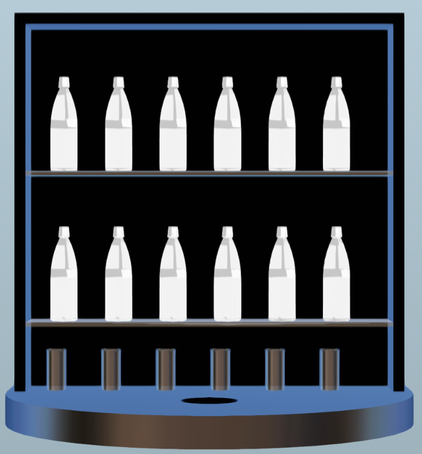
\includegraphics[width=0.5\linewidth]{pictures/bar_inventor.png}}
\captionof{figure}{Sketch of the bar}\label{fig:bar_inventor}%      only if needed  
\end{minipage}

In our approach we planed a bar with Adobe Inventor, which was designed with two plexiglass shelves each with room for six bottles. Under the lowermost shelf we planed to place the cocktail glasses, the ice bucket and the cocktail shaker. Behind the plexiglass shelves we arranged LED strips, which made it possible to illuminated each bottle on its own.
In the bottom plate of the bar, which consists of two plates with a cavity between them, we integrated a weight measuring module, so that the bar is able to know how much of each ingredient the user already filled in the glass. To do so the bar uses LED strips under the weight module to give exacted feedback.  
Furthermore the cavity of the bottom plate made it possible to stow all electronics inside the bar so that the user does not see any wiring unless the raspberry pi surface. On this surface we wanted to give little instructions for each step in the mixing process of the selected cocktail.

\begin{figure}[htbp] 
  \centering
     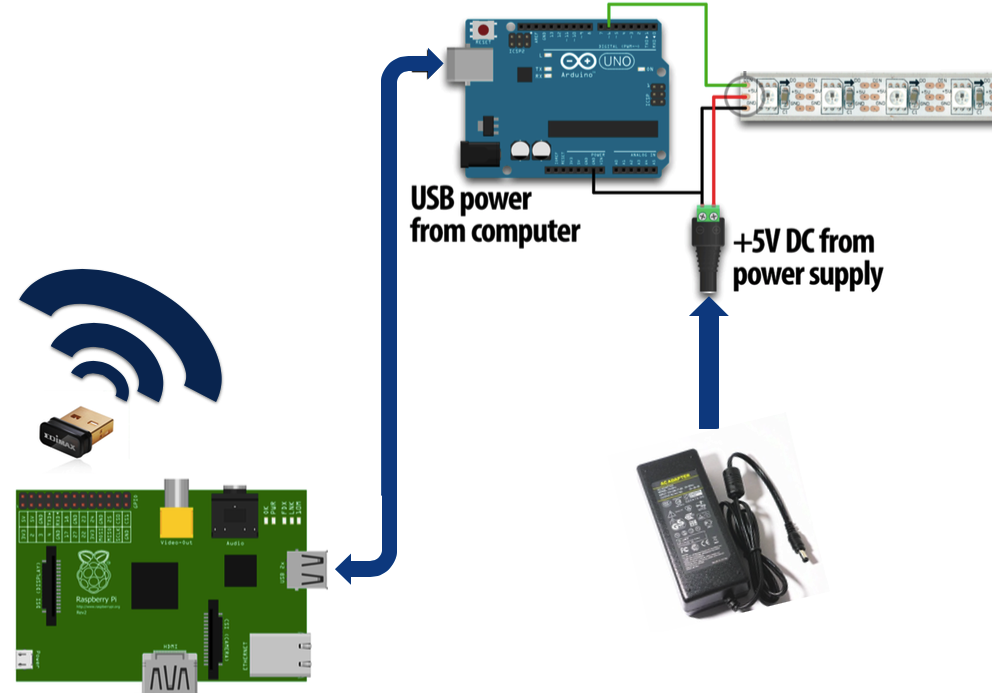
\includegraphics[width=0.7\linewidth]{pictures/technical.png}
  \caption{Technical sketch}
  \label{fig:technical}
\end{figure}

In the first technical sketch we used a Raspberry Pi creating a WiFi network and running a web server providing the website of the bar. This Raspberry Pi was connected via a serial connection over a USB cable to a Arduino Uno. To this micro controller we wanted to connect the LED strips and the weight measuring module.

\section{Hardware Construction}
\subsection{Woodwork}

\begin{minipage}{\linewidth}% to keep image and caption on one page
\makebox[\linewidth]{%        to center the image
  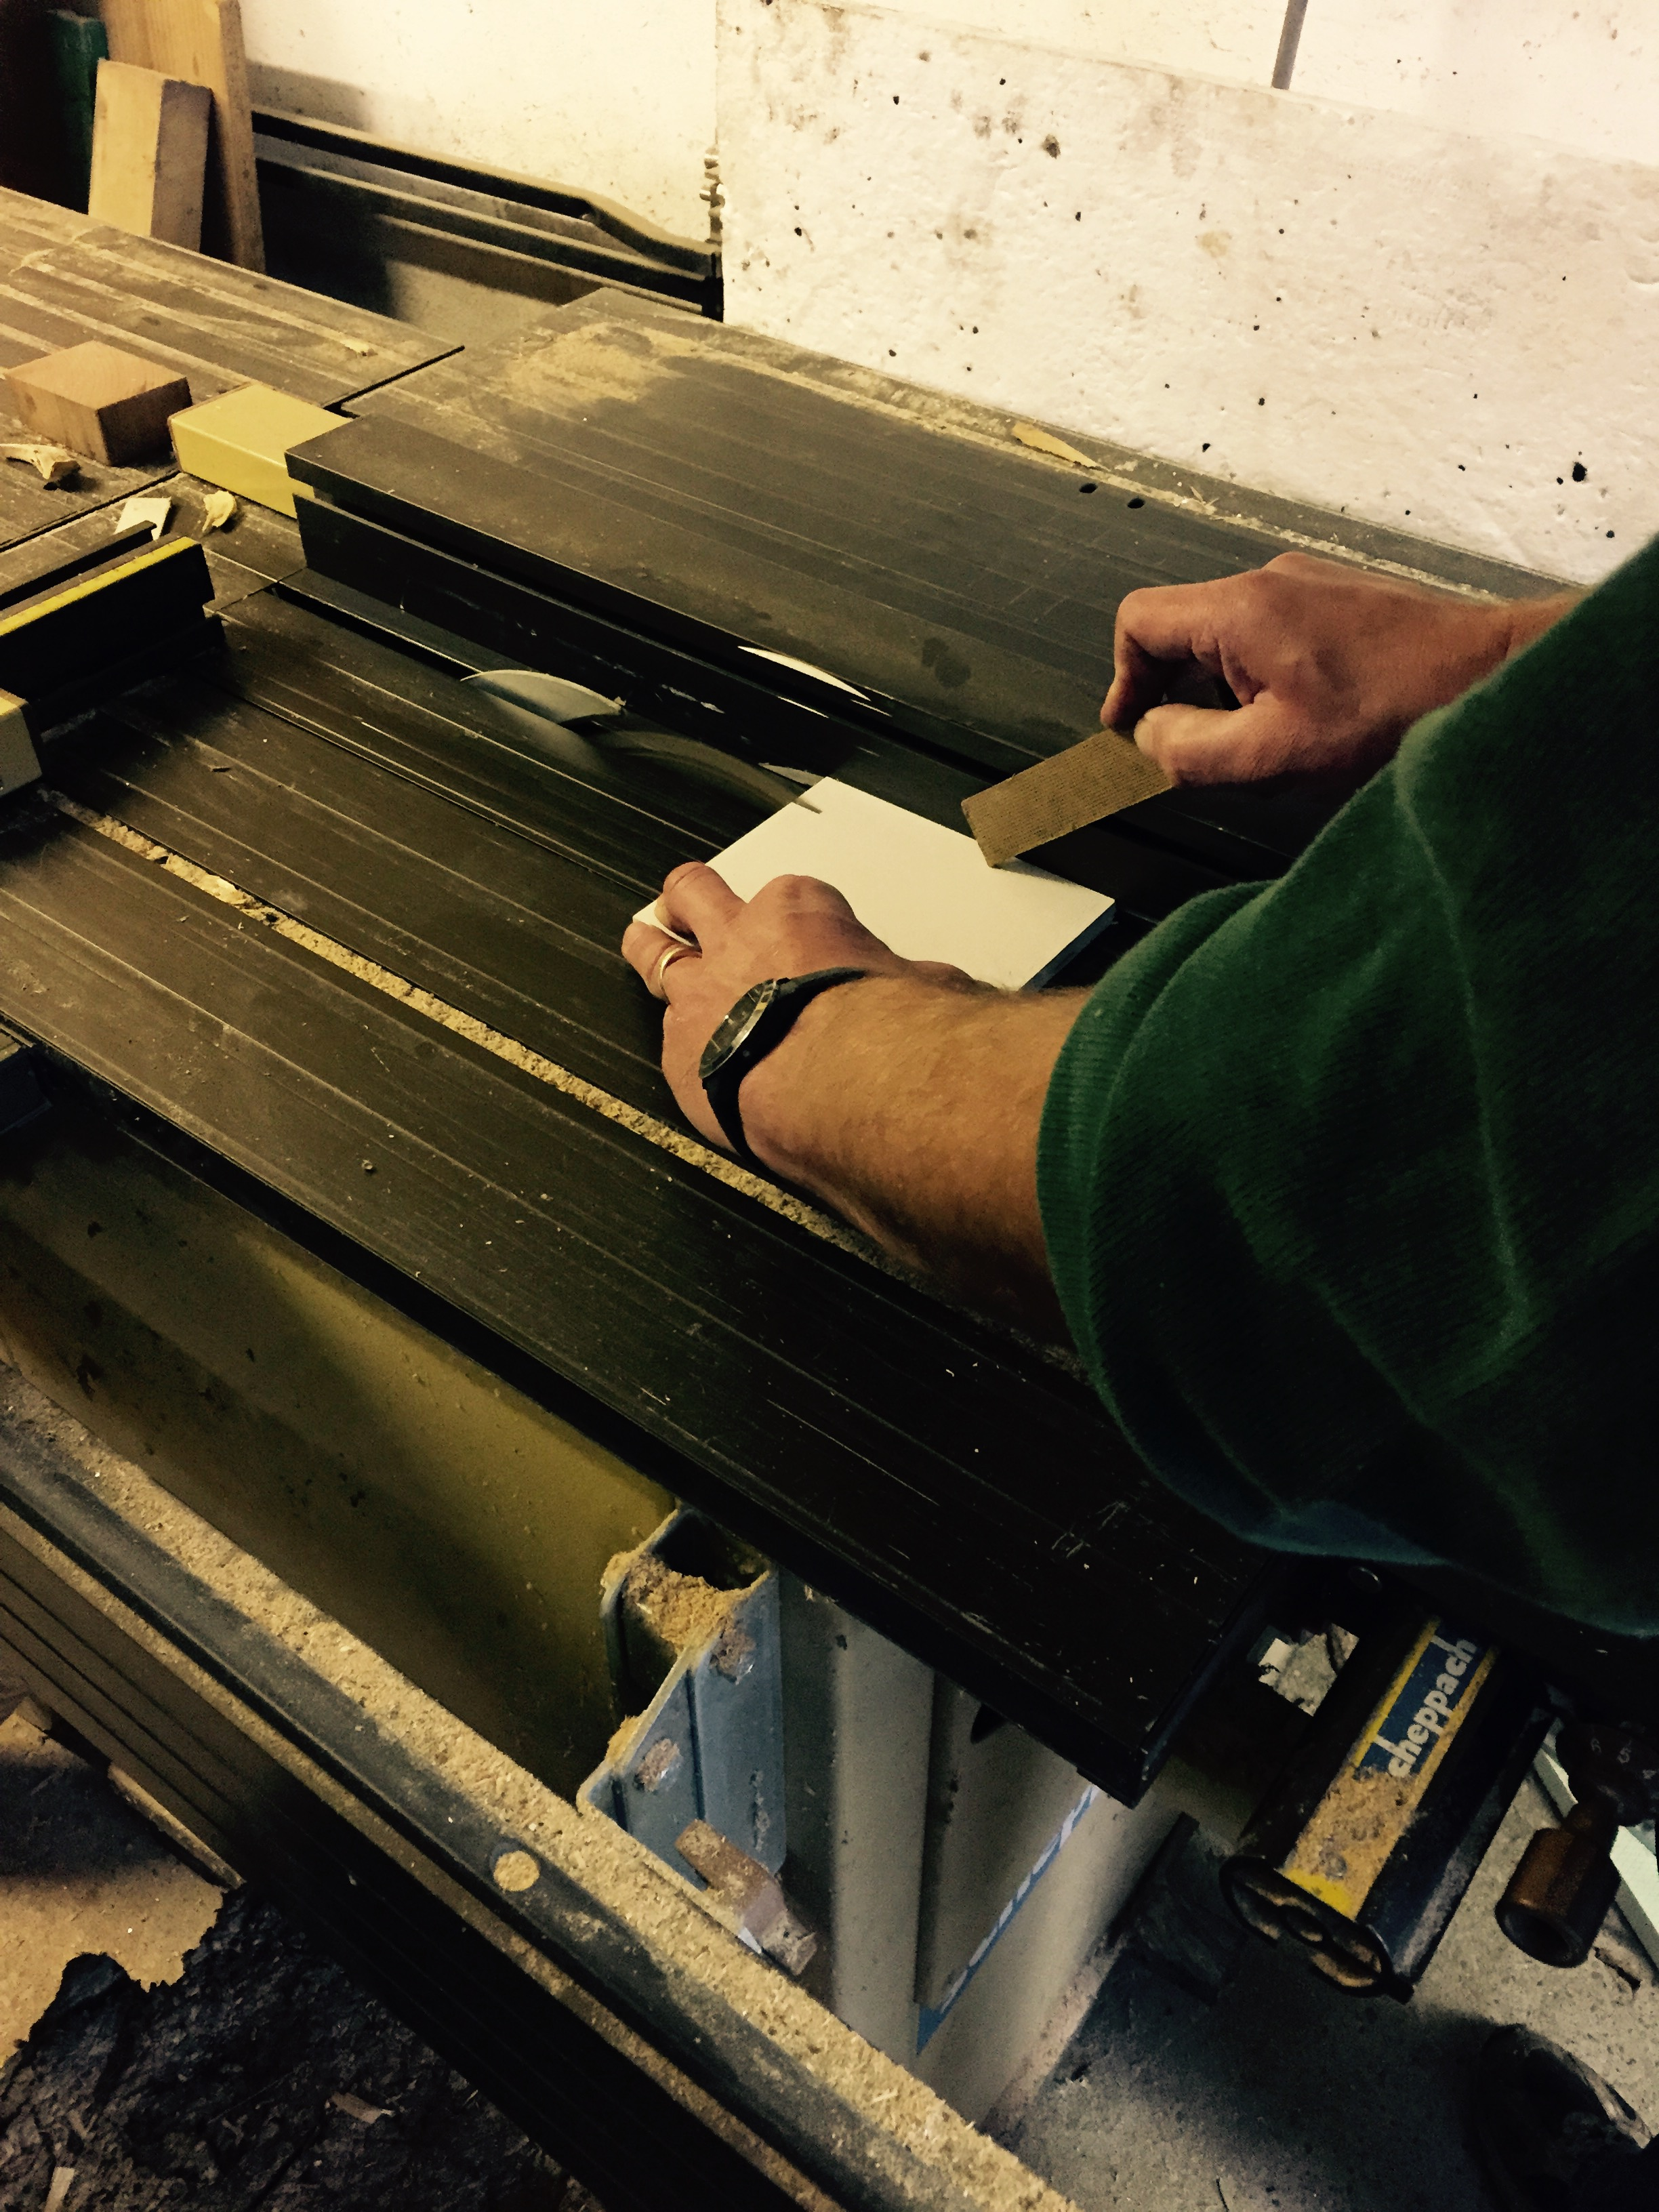
\includegraphics[width=0.7\linewidth]{pictures/cutting_wood.jpg}}
\captionof{figure}{Cutting of the wood}\label{fig:cutting_wood}%      only if needed  
\end{minipage}


After planning the rack and the shelves of the bar, we calculated the amount of wood we would need to build it. In a next step we had to cut the wood we bought into the right pieces. For the rounding of the rack bottom we contacted a local carpenter since we did not have the right instruments for doing this difficult cuts properly. The other small pieces were cut with a buzz saw as you can see in figure \ref{fig:cutting_wood}.

\begin{minipage}{\linewidth}% to keep image and caption on one page
\makebox[\linewidth]{%        to center the image
  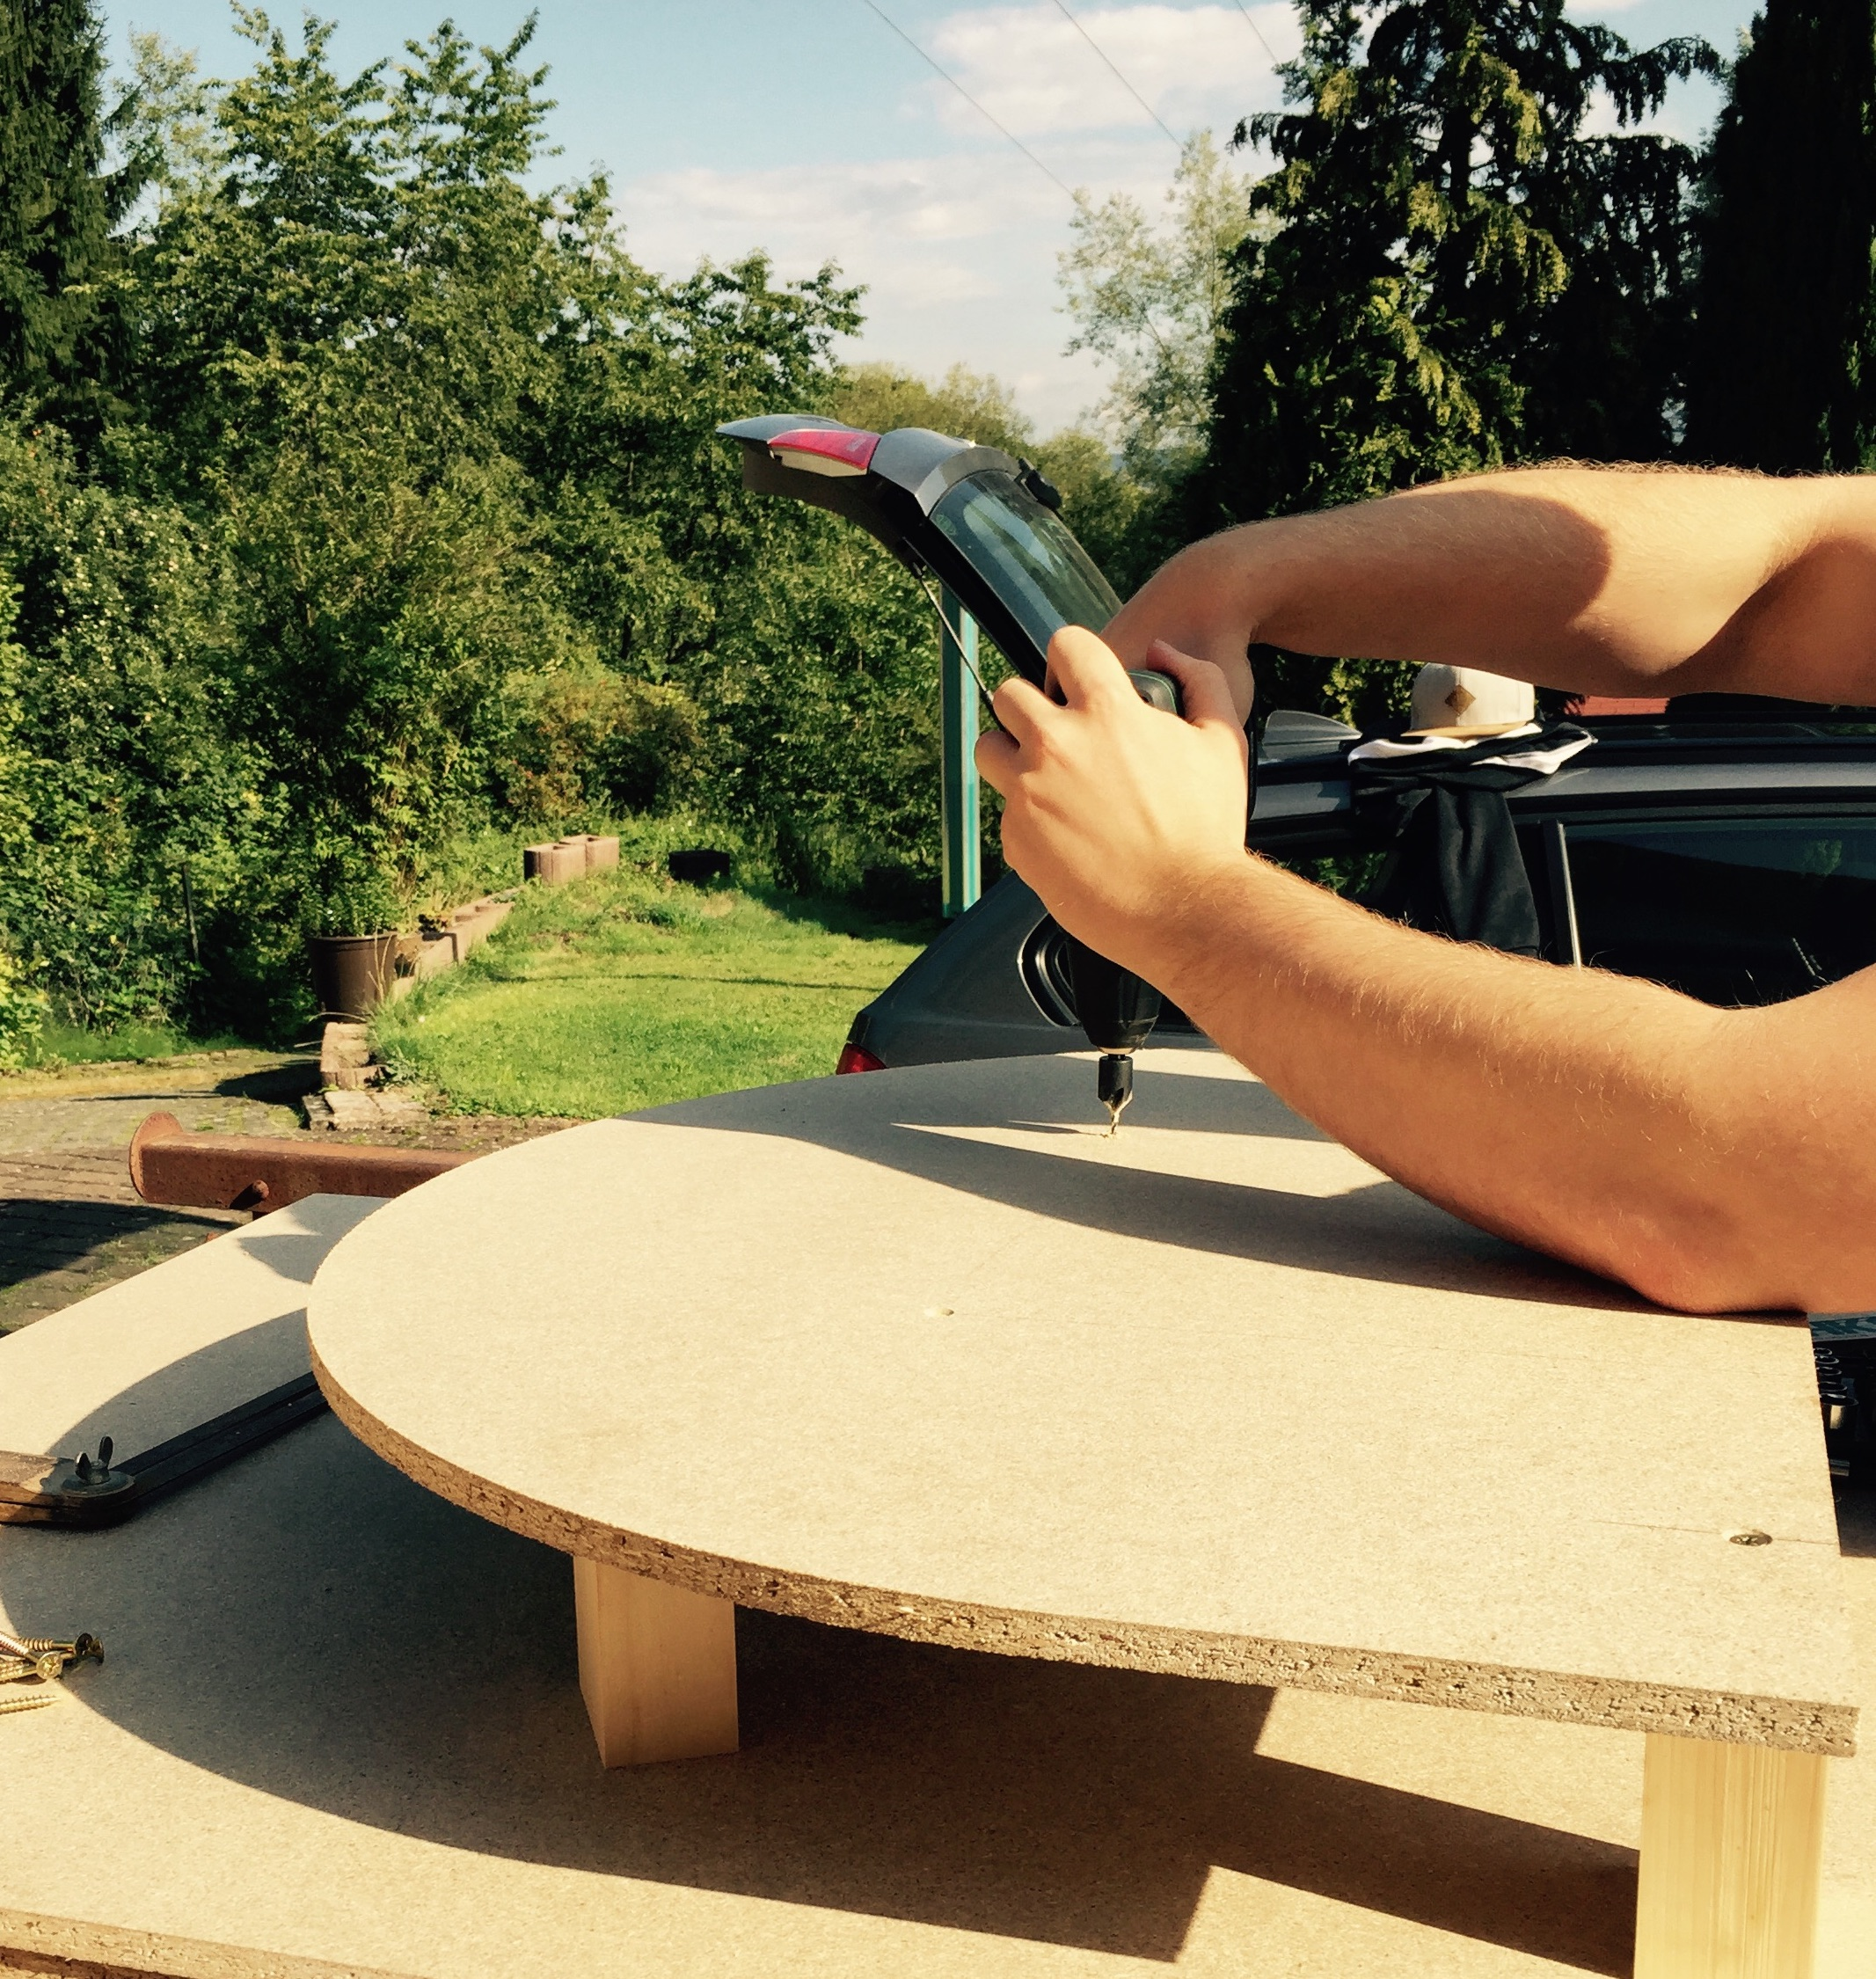
\includegraphics[width=0.5\linewidth]{pictures/assembling.jpg}}
\captionof{figure}{Assembling of the rack}\label{fig:assembling}%      only if needed  
\end{minipage}

When all pieces of the rack were fitted, we started to assemble the rack. Therefore we used screws and wood glue so that the bar would keep stable. Figure \ref{fig:assembling} shows how the base plate is screwed together.

\begin{minipage}{\linewidth}% to keep image and caption on one page
\makebox[\linewidth]{%        to center the image
  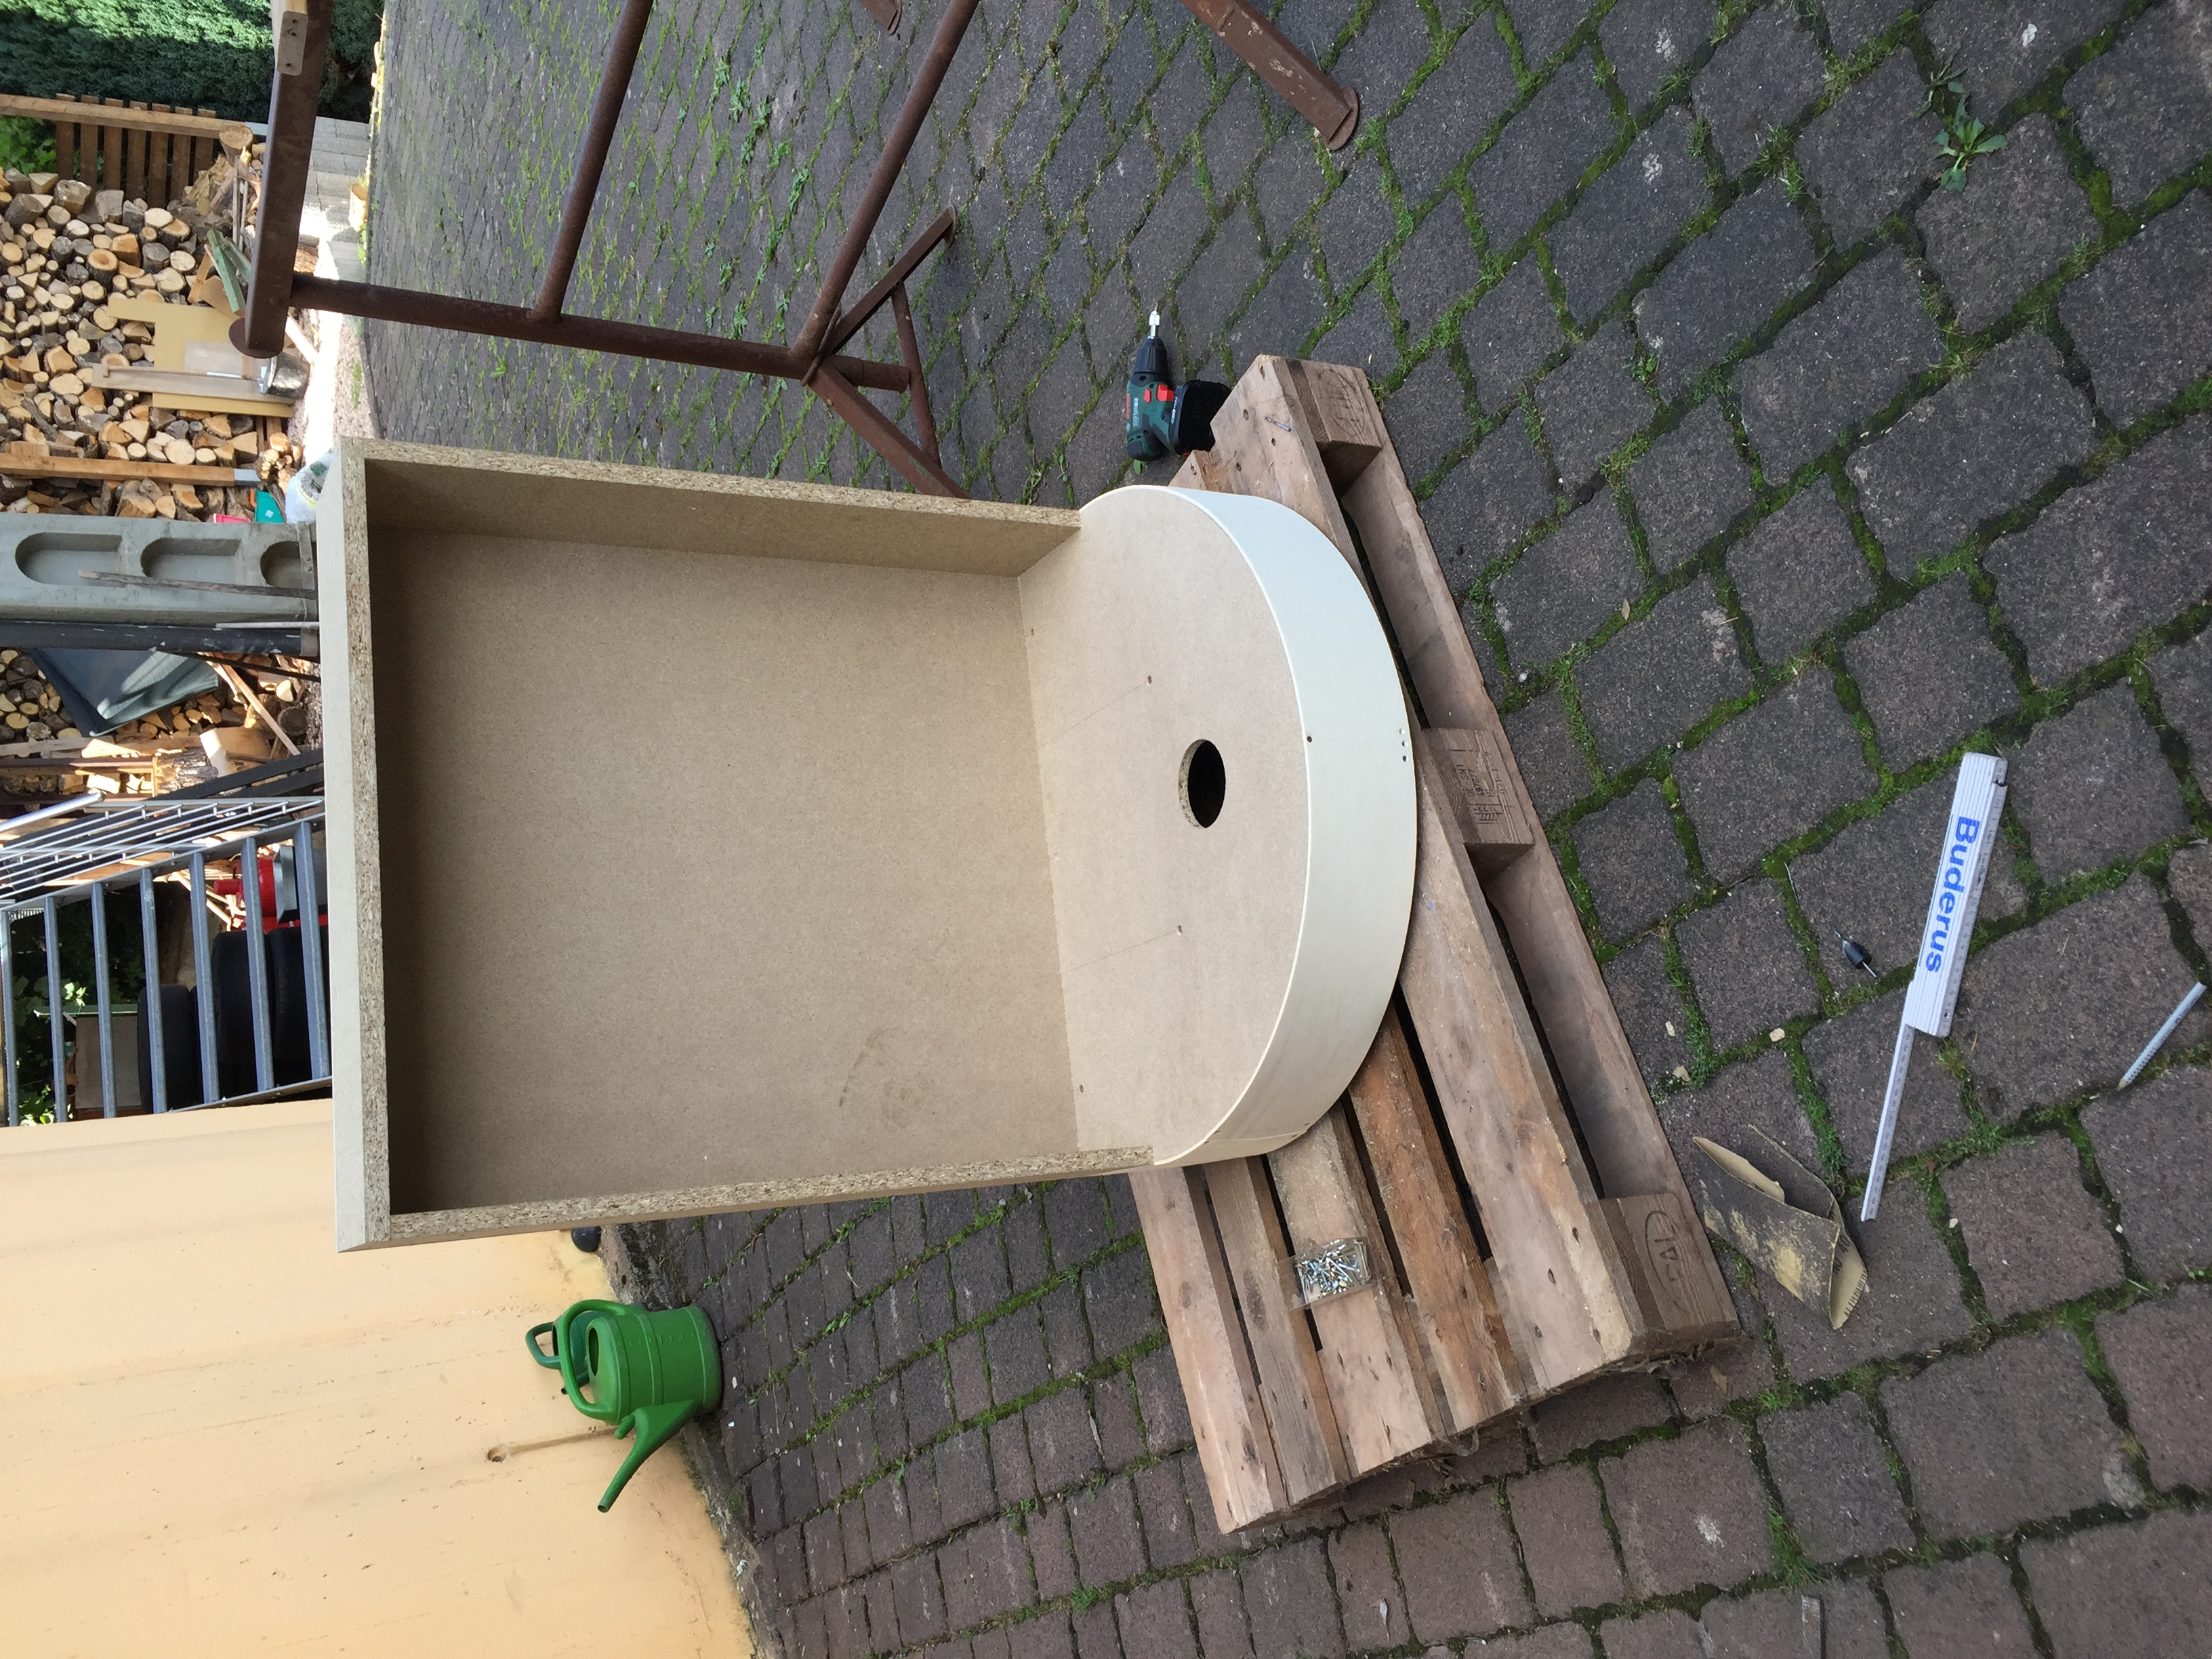
\includegraphics[width=0.6\linewidth, angle =270]{pictures/rack2.jpg}}
\captionof{figure}{Framing of the rack}\label{fig:framing}%      only if needed  
\end{minipage}


The finished framing of the rack is shown in figure \ref{fig:framing}. This picture also illustrates that we did the panelling between the two base plates with 4 mm poplar wood because this is to thin and flexible that it can be bend.

\begin{minipage}{\linewidth}% to keep image and caption on one page
\makebox[\linewidth]{%        to center the image
  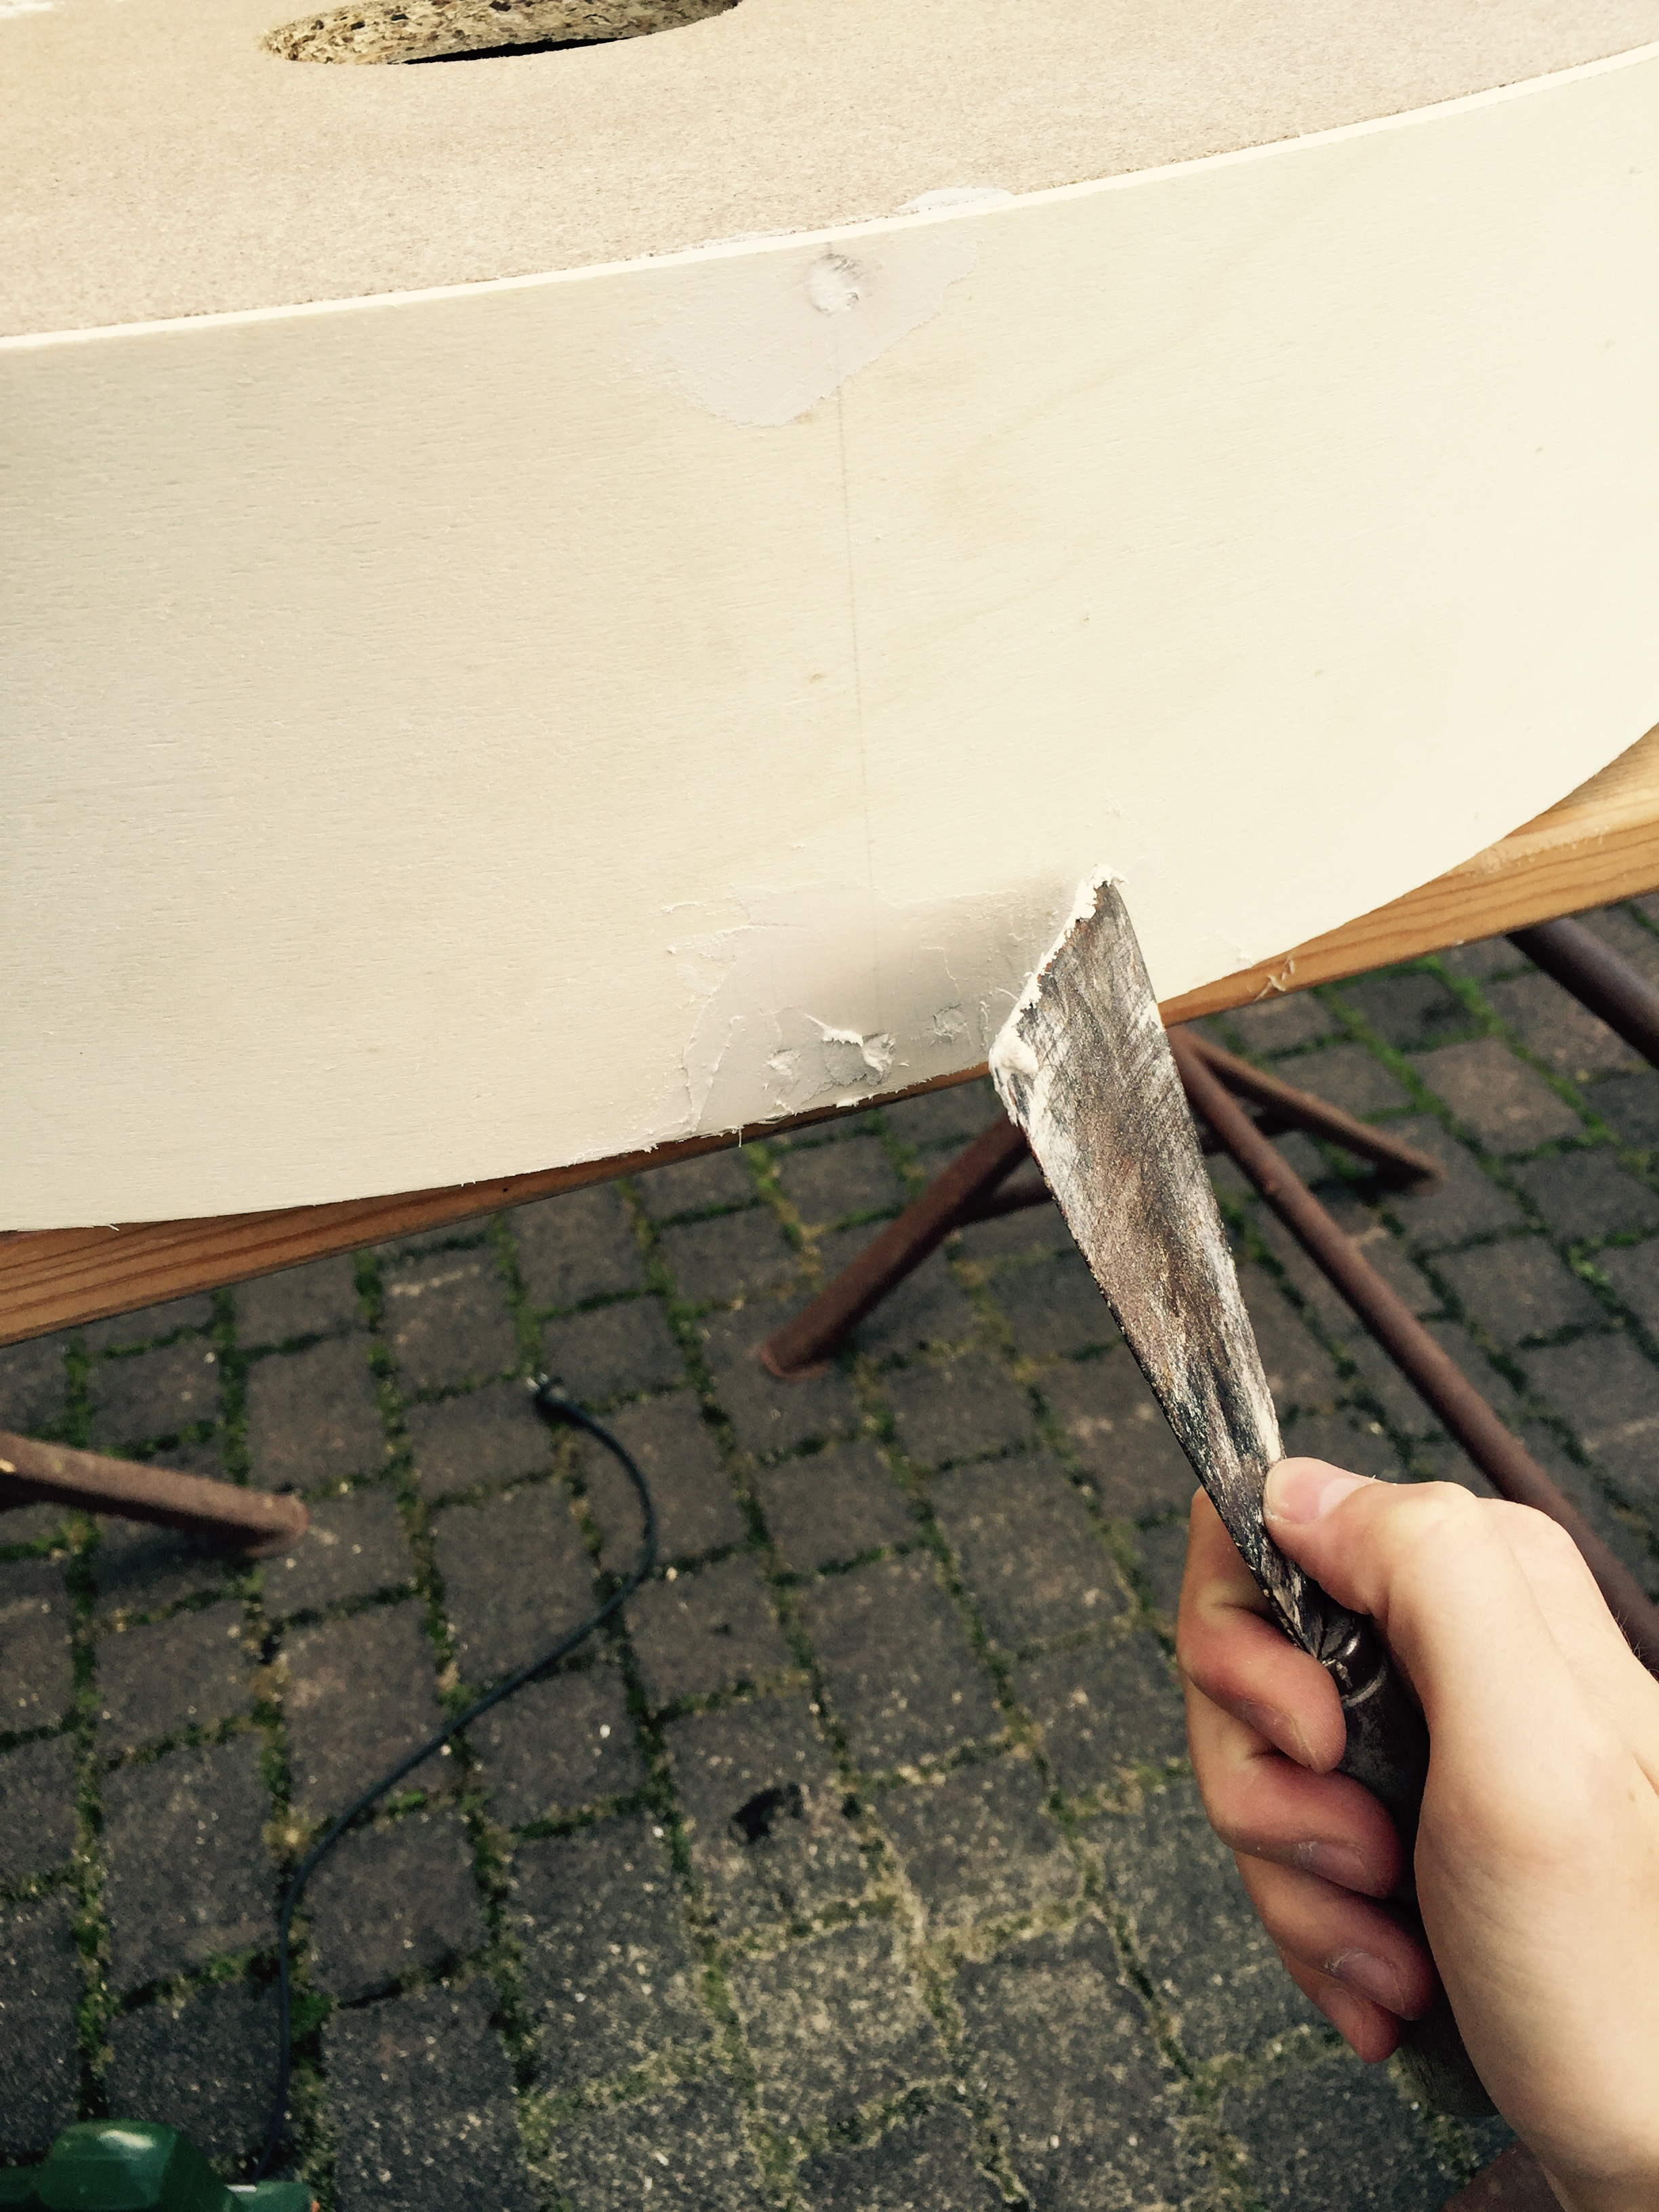
\includegraphics[width=0.55\linewidth]{pictures/filling.jpg}}
\captionof{figure}{Filling of the screw wholes}\label{fig:filling}%      only if needed  
\end{minipage}


For deriving a smooth surface of the rack, we filled all screw wholes with filler. Since we used plywood, we also filled the edges of the rack, so that it is easier to prime and paint the bar. 

\begin{minipage}{\linewidth}% to keep image and caption on one page
\makebox[\linewidth]{%        to center the image
  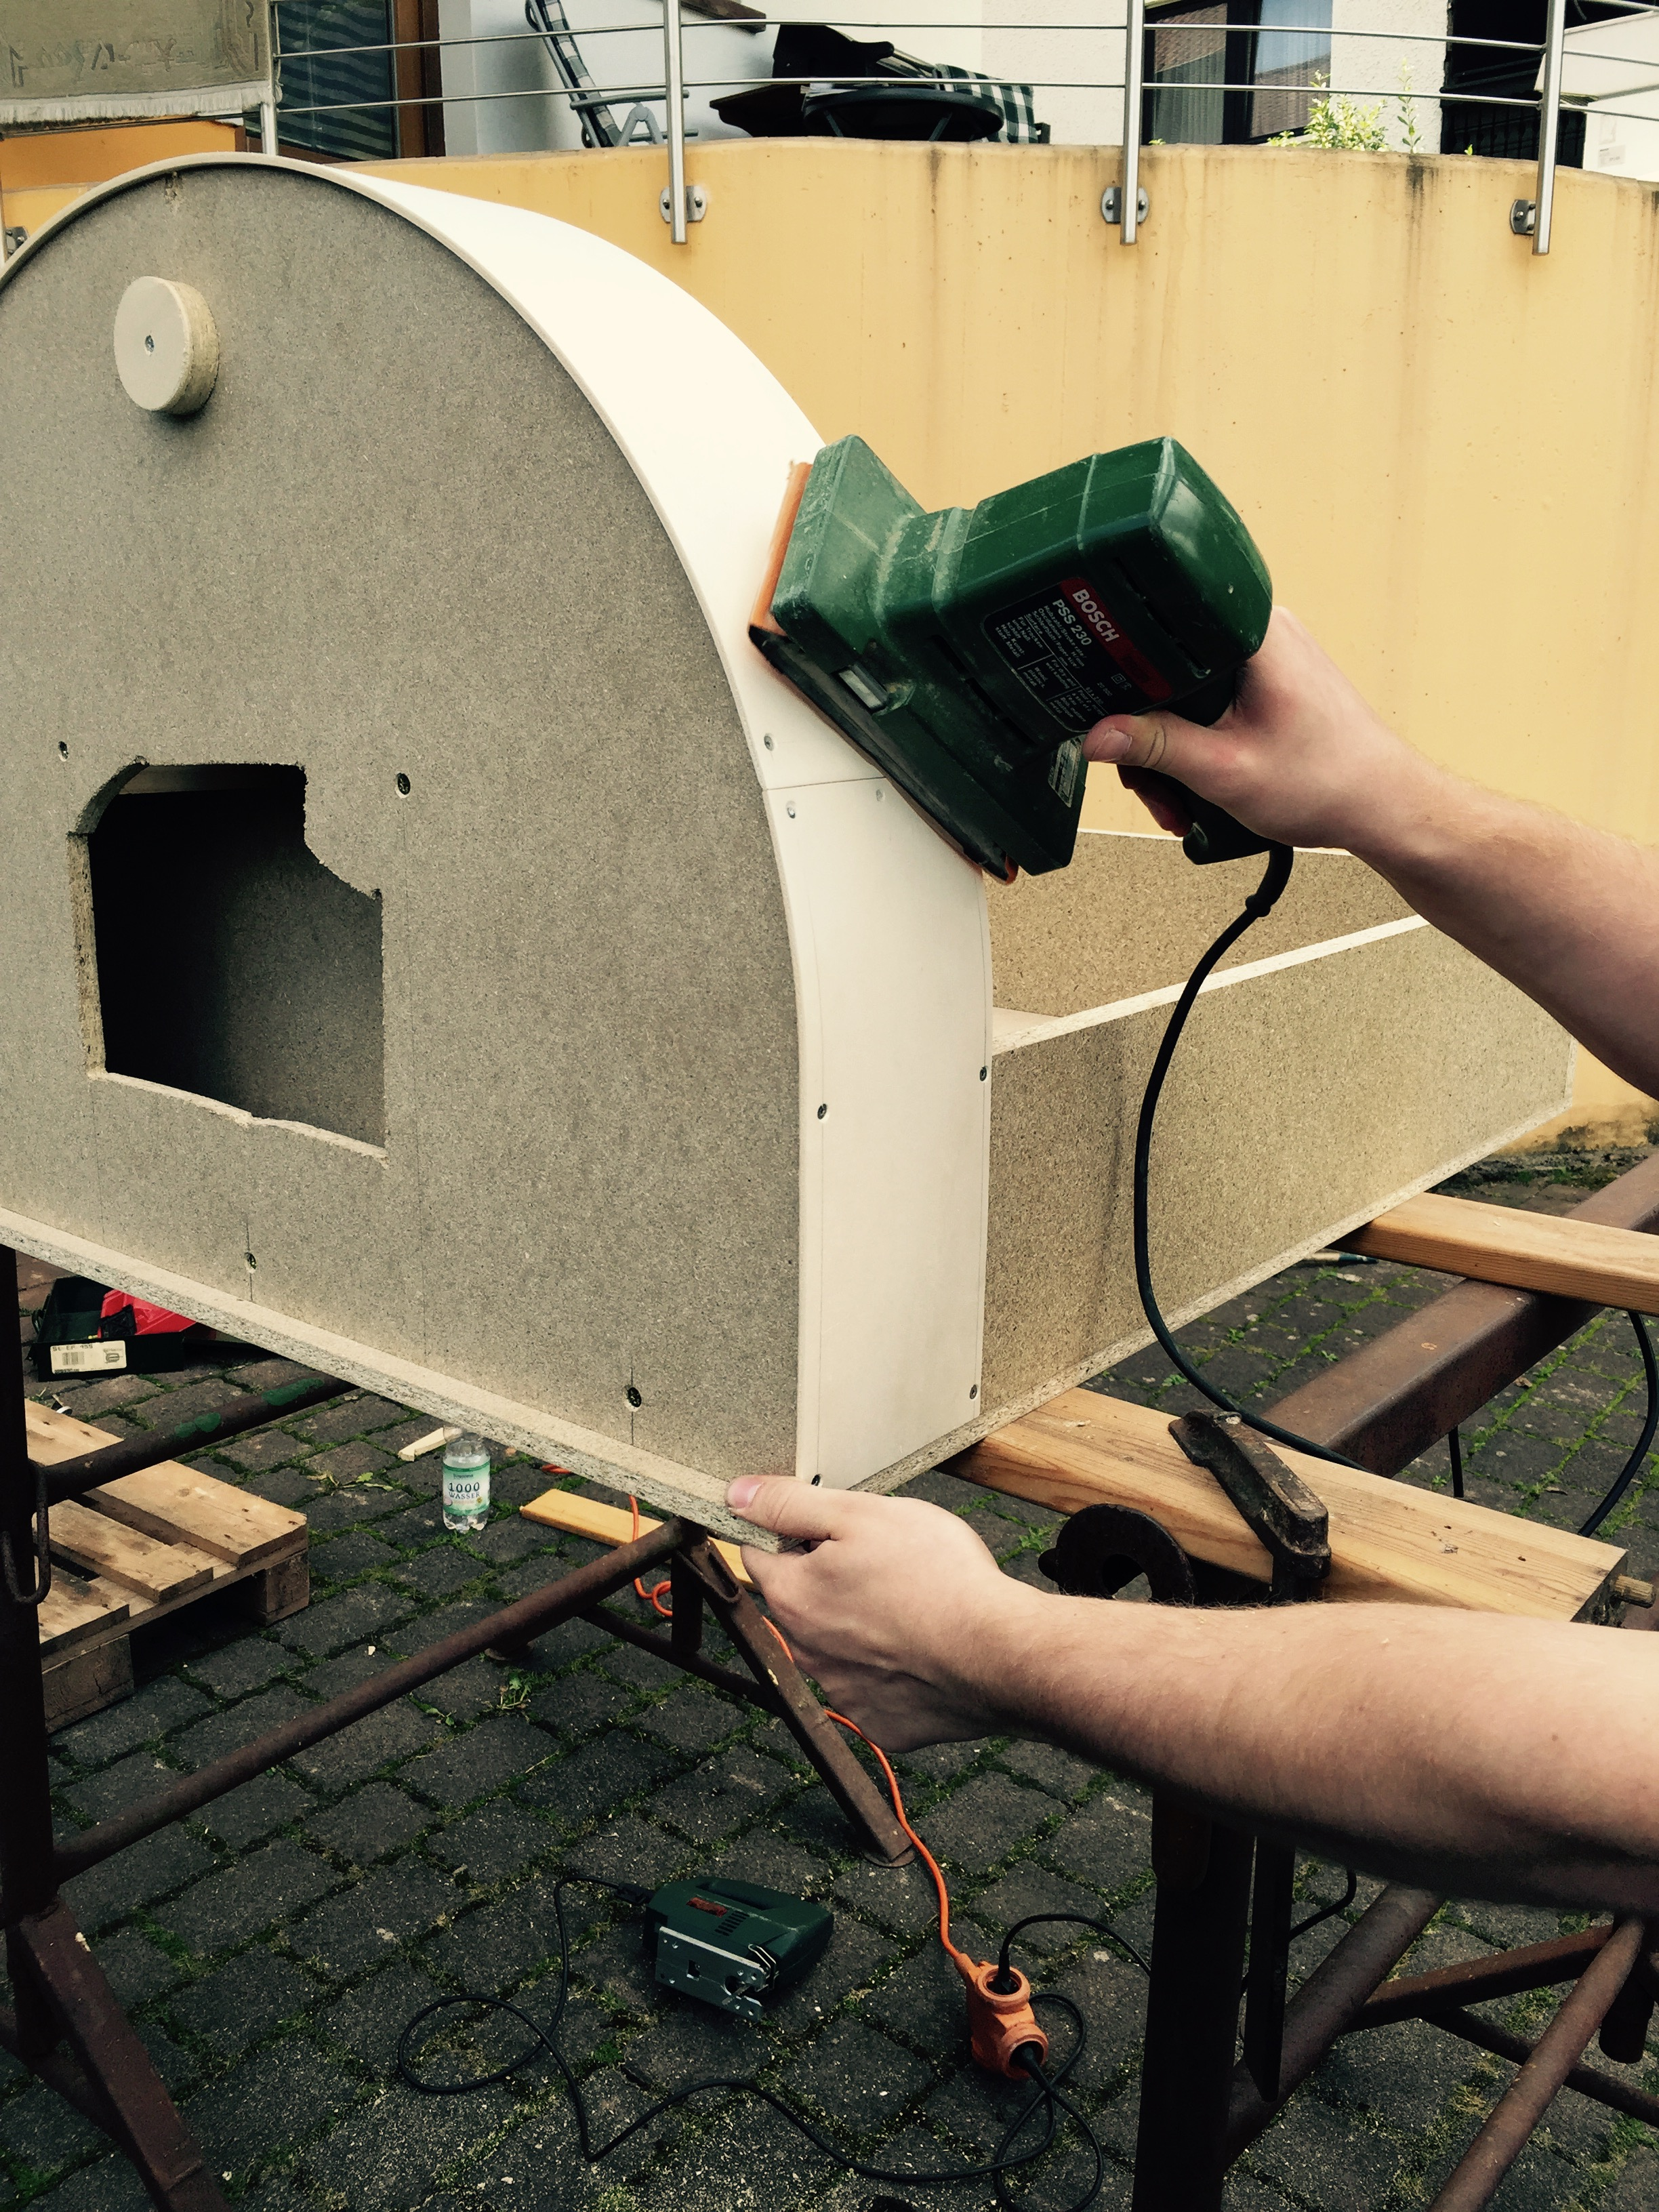
\includegraphics[width=0.5\linewidth]{pictures/polishing.jpg}}
\captionof{figure}{Polishing the rack}\label{fig:polishing}%      only if needed  
\end{minipage}


In a next step we polished the bar since had to remove the needless filler and roughen the wood. This work step can be seen in figure \ref{fig:polishing}

\begin{minipage}{\linewidth}% to keep image and caption on one page
\makebox[\linewidth]{%        to center the image
   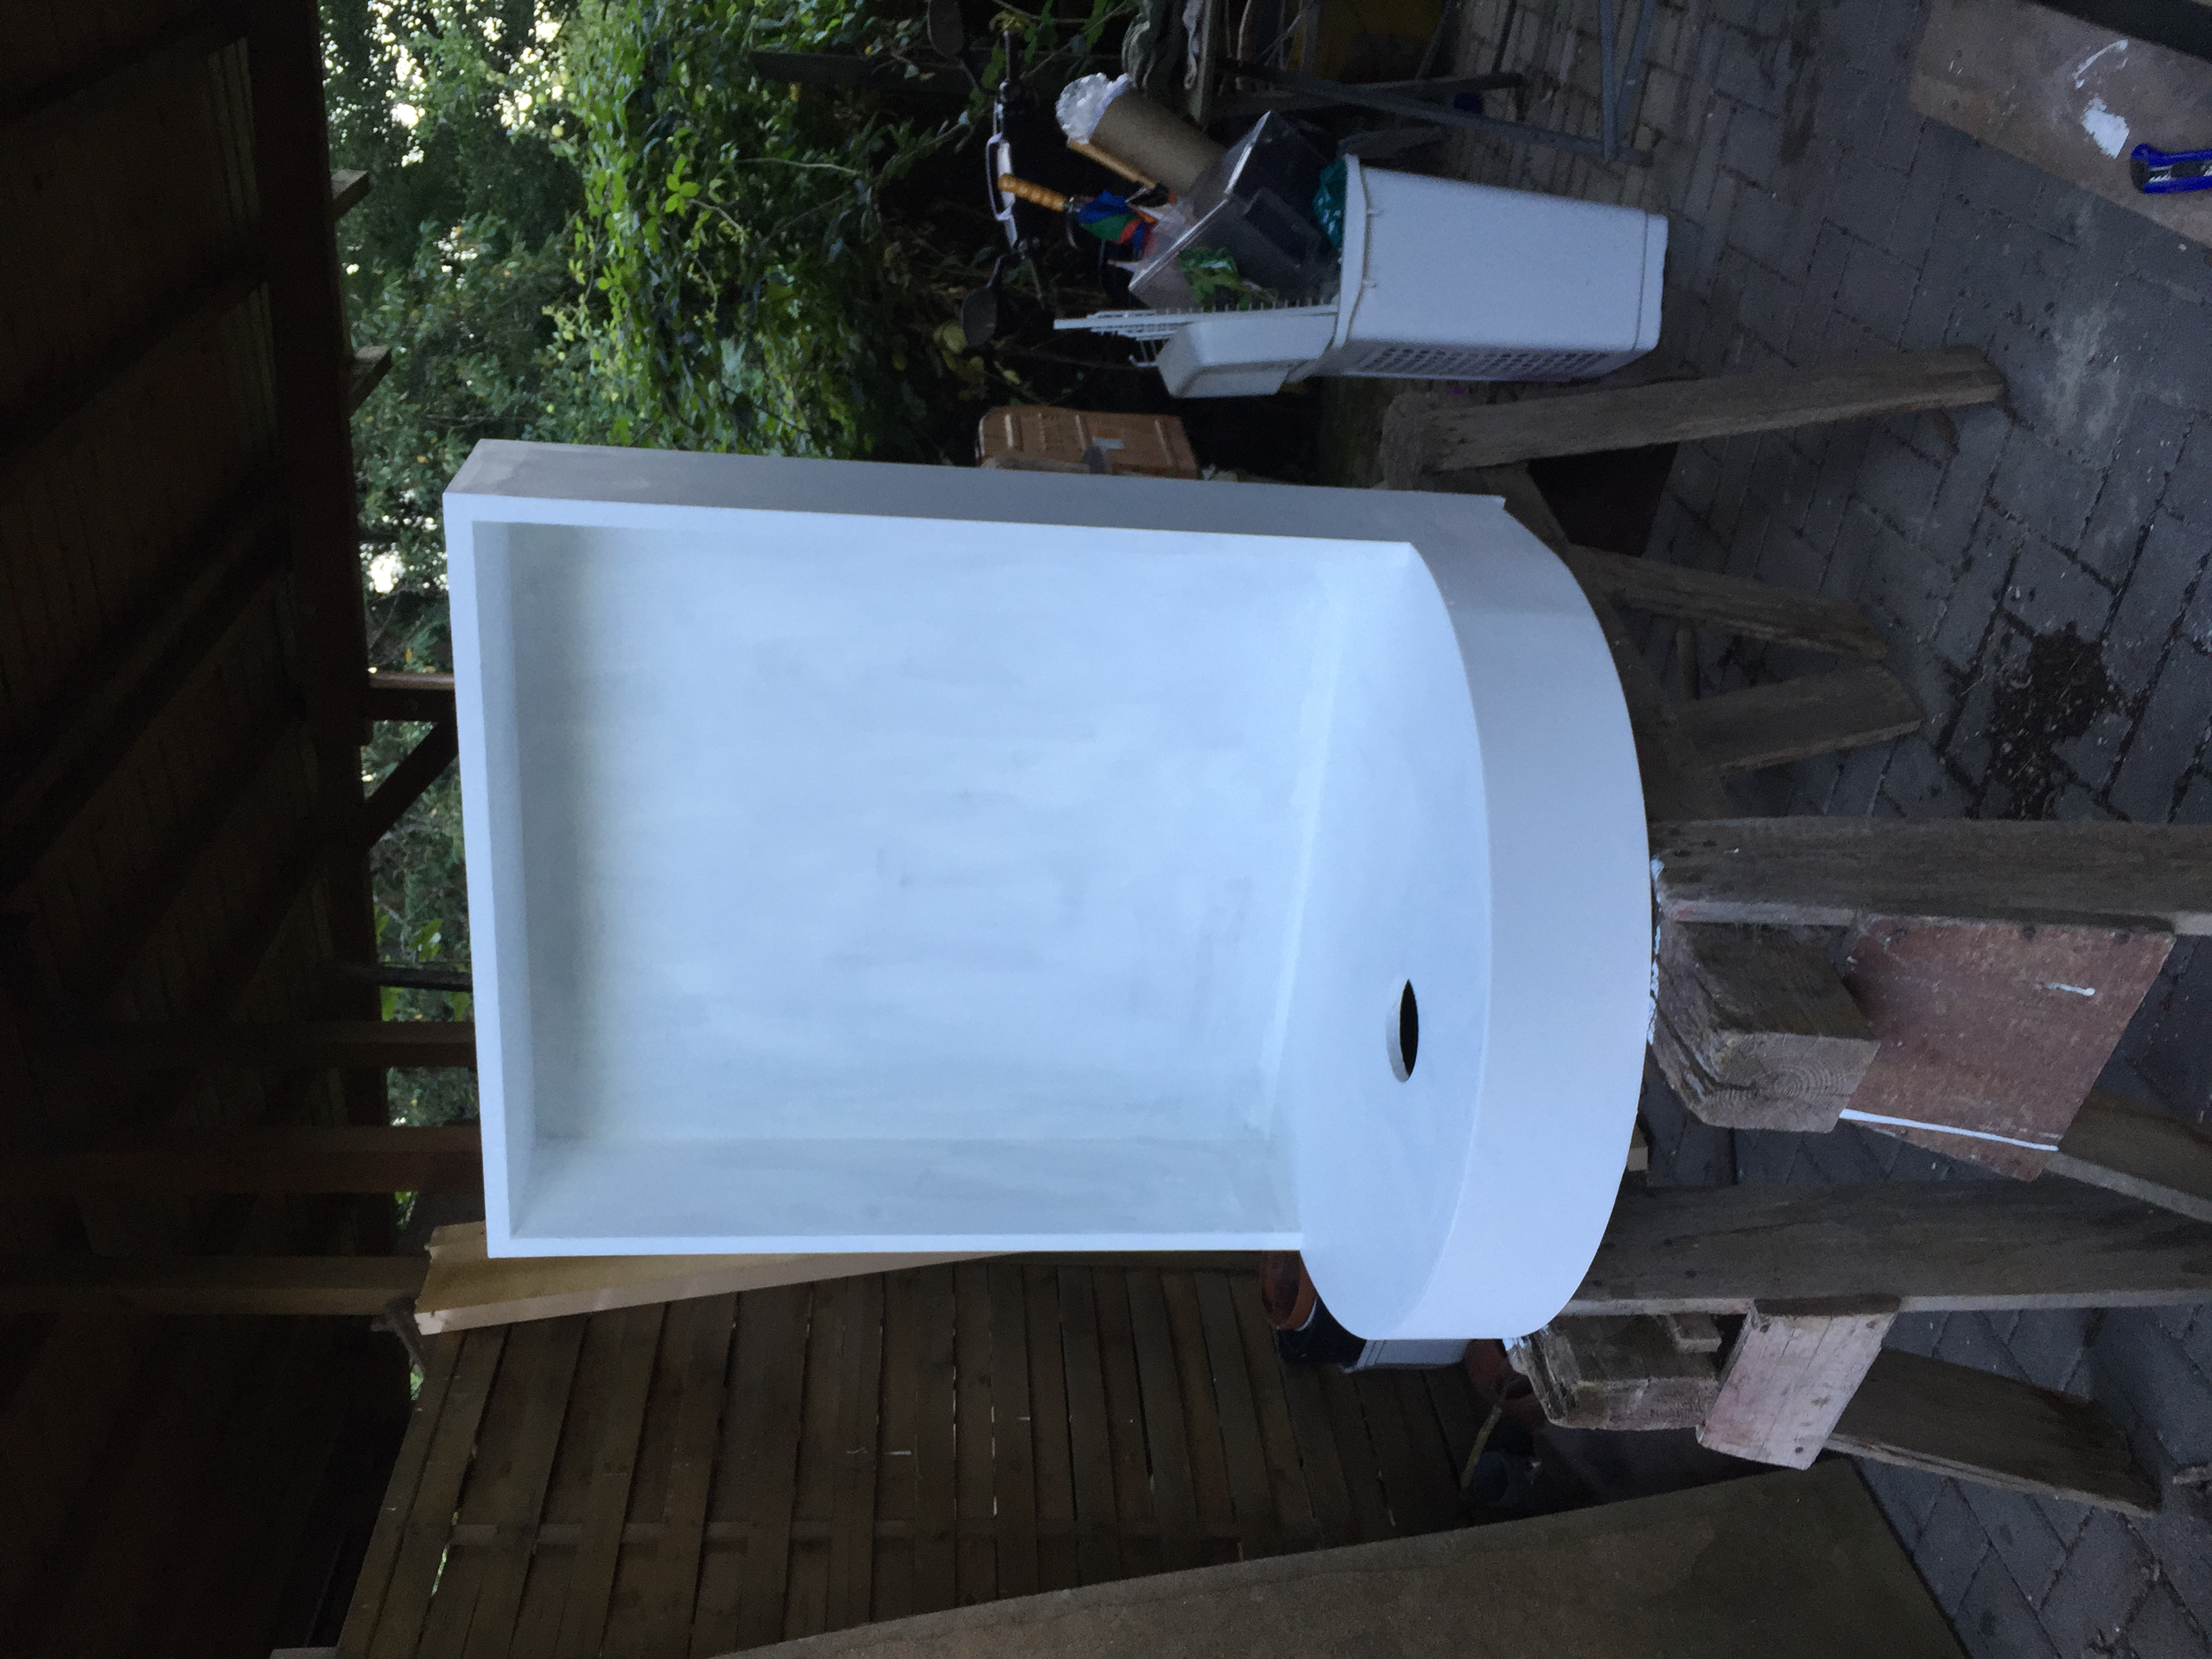
\includegraphics[width=0.6\linewidth, angle =270]{pictures/rack3.jpg}}
\captionof{figure}{The primed rack}\label{fig:priming}%      only if needed  
\end{minipage}
 

After polishing and cleaning the rack with compressed air, we were able to prime the rack. This is important since primer creates a smooth and consistent layer for the paint.


\subsection{Plexiglass Shelves}

\begin{minipage}{\linewidth}% to keep image and caption on one page
\makebox[\linewidth]{%        to center the image
   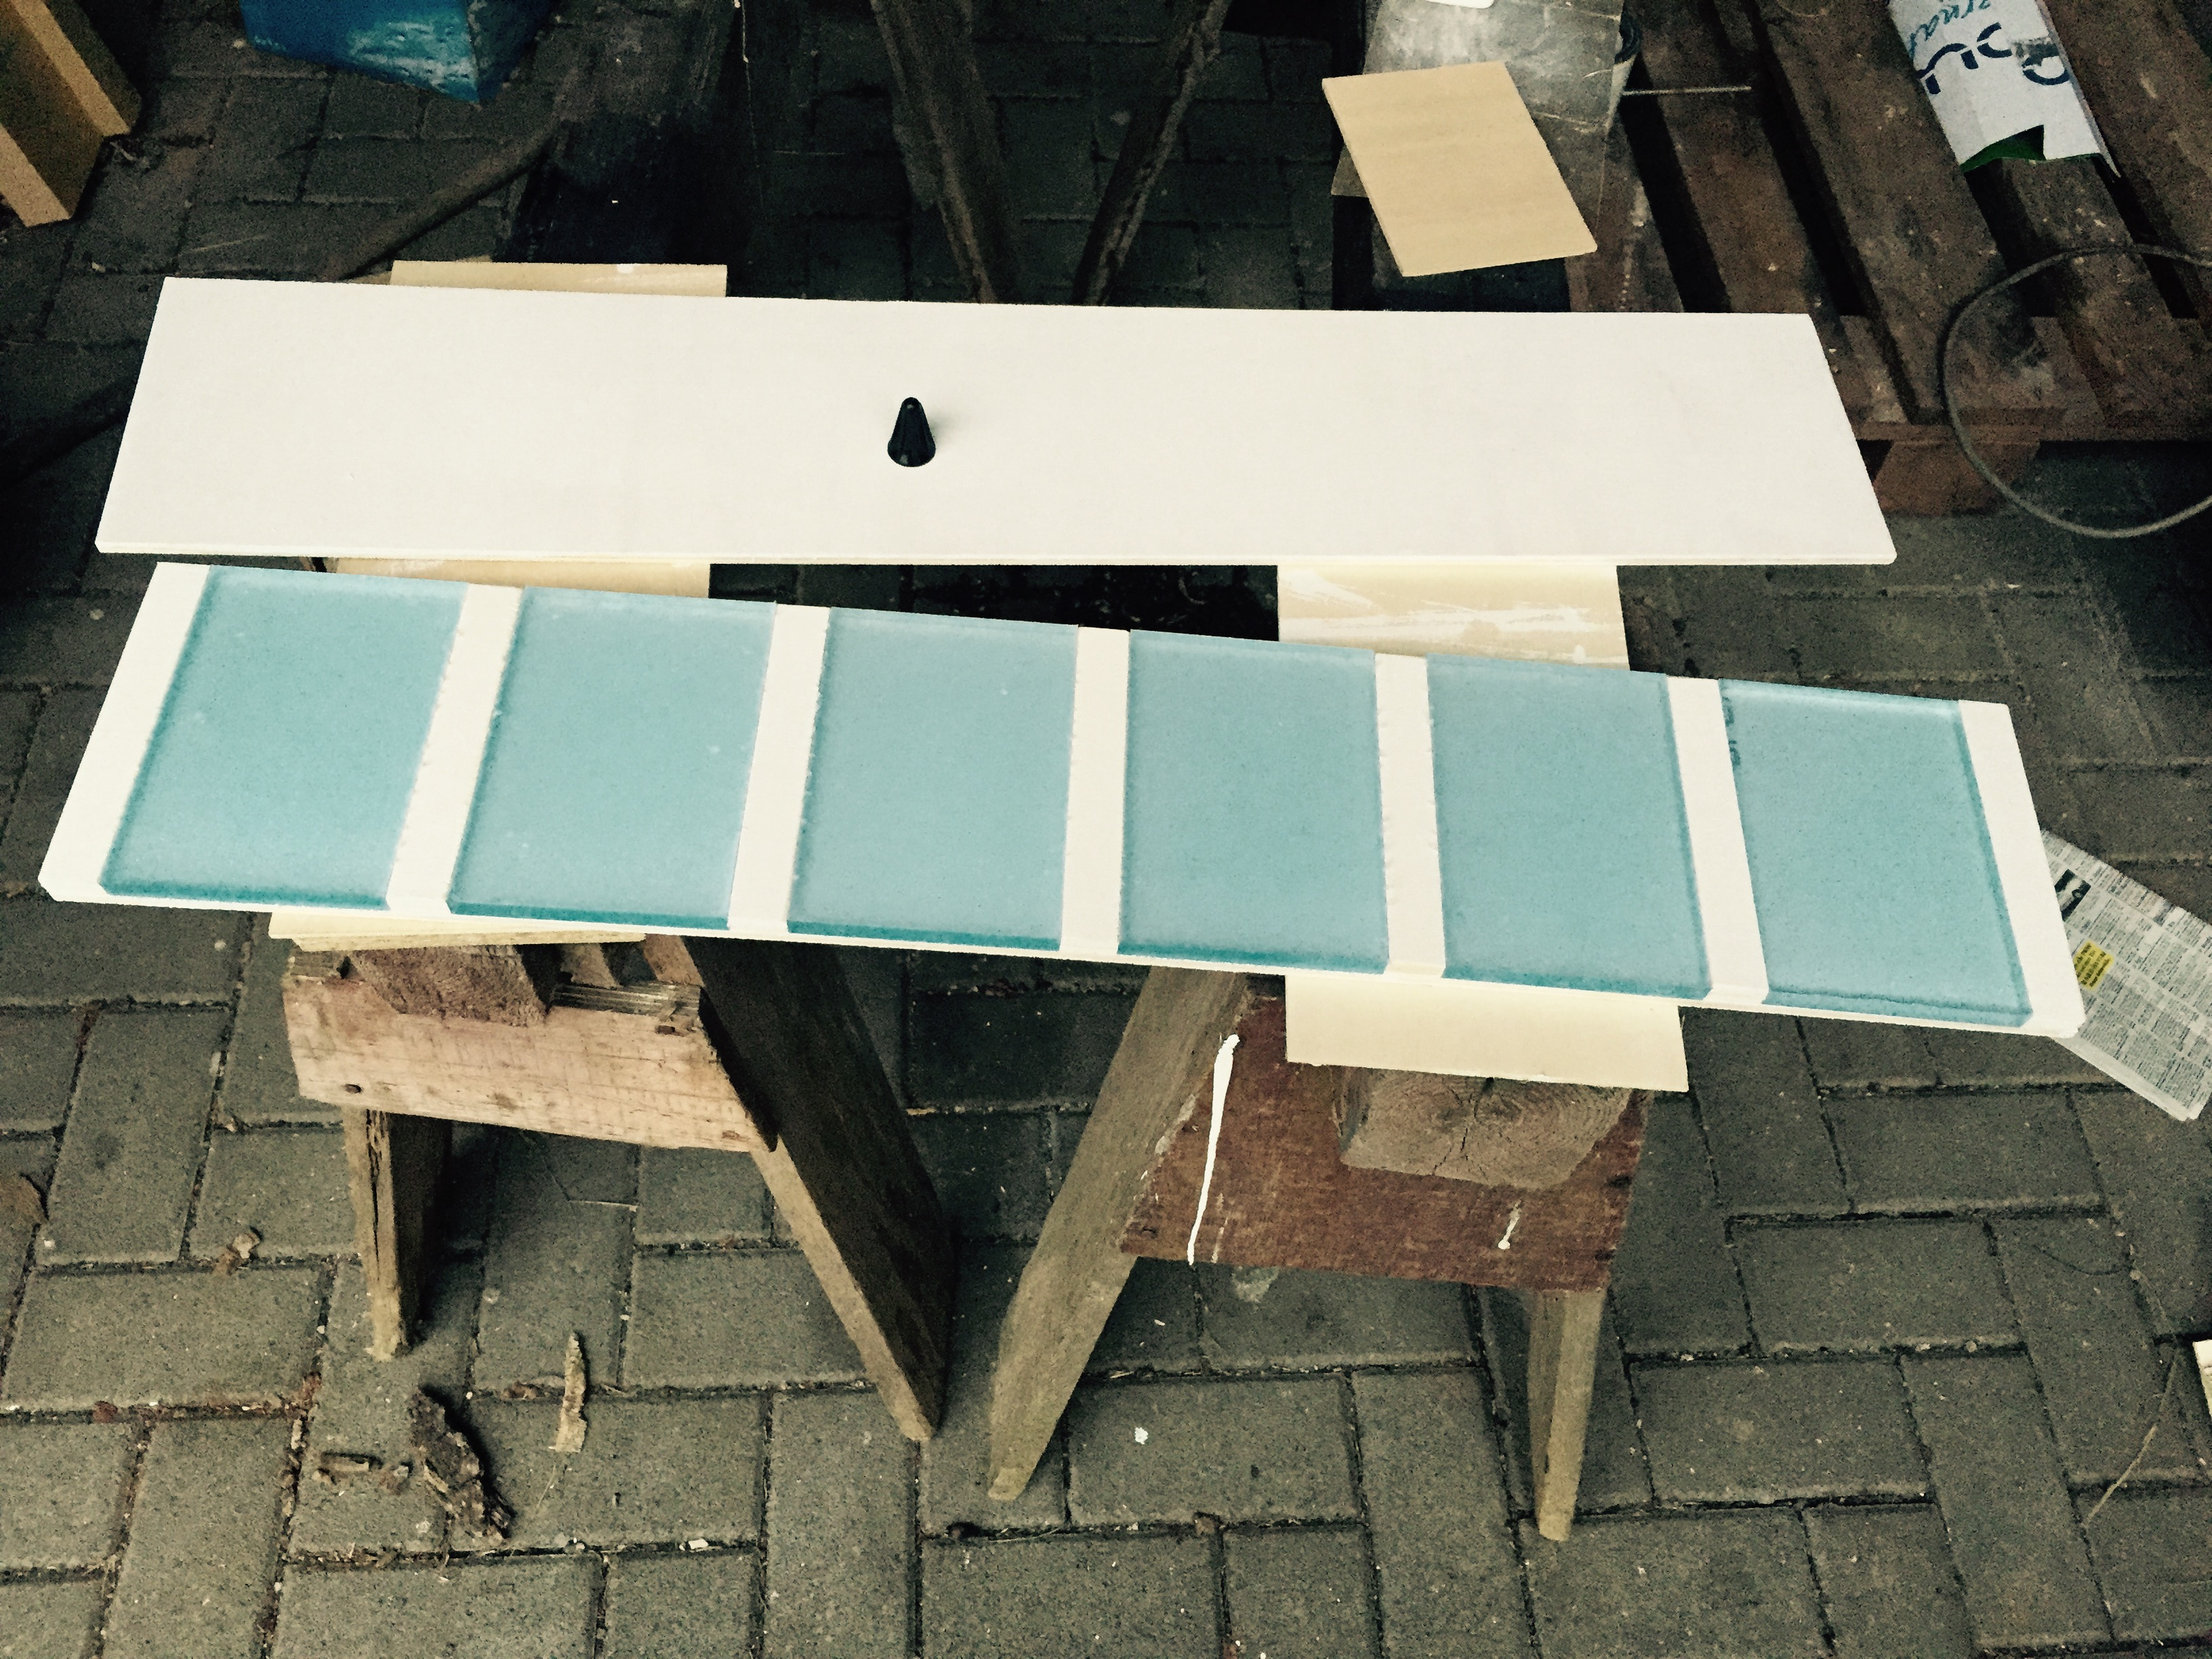
\includegraphics[width=0.5\linewidth]{pictures/plexiglass.jpg}}
\captionof{figure}{Building the shelves}\label{fig:building_shelves}%      only if needed  
\end{minipage}

The initial design planed that the two shelves only consisted of two full pelxiglass plates. At the beginning of the design process we tested this approach and noticed that the illumination of the bottles was not as good as expected since the light scattered through the whole shelve when we only lighted one bottle. Therefore we redesigned the two shelves as you can see in figure \ref{fig:building_shelves}. 

\begin{minipage}{\linewidth}% to keep image and caption on one page
\makebox[\linewidth]{%        to center the image
   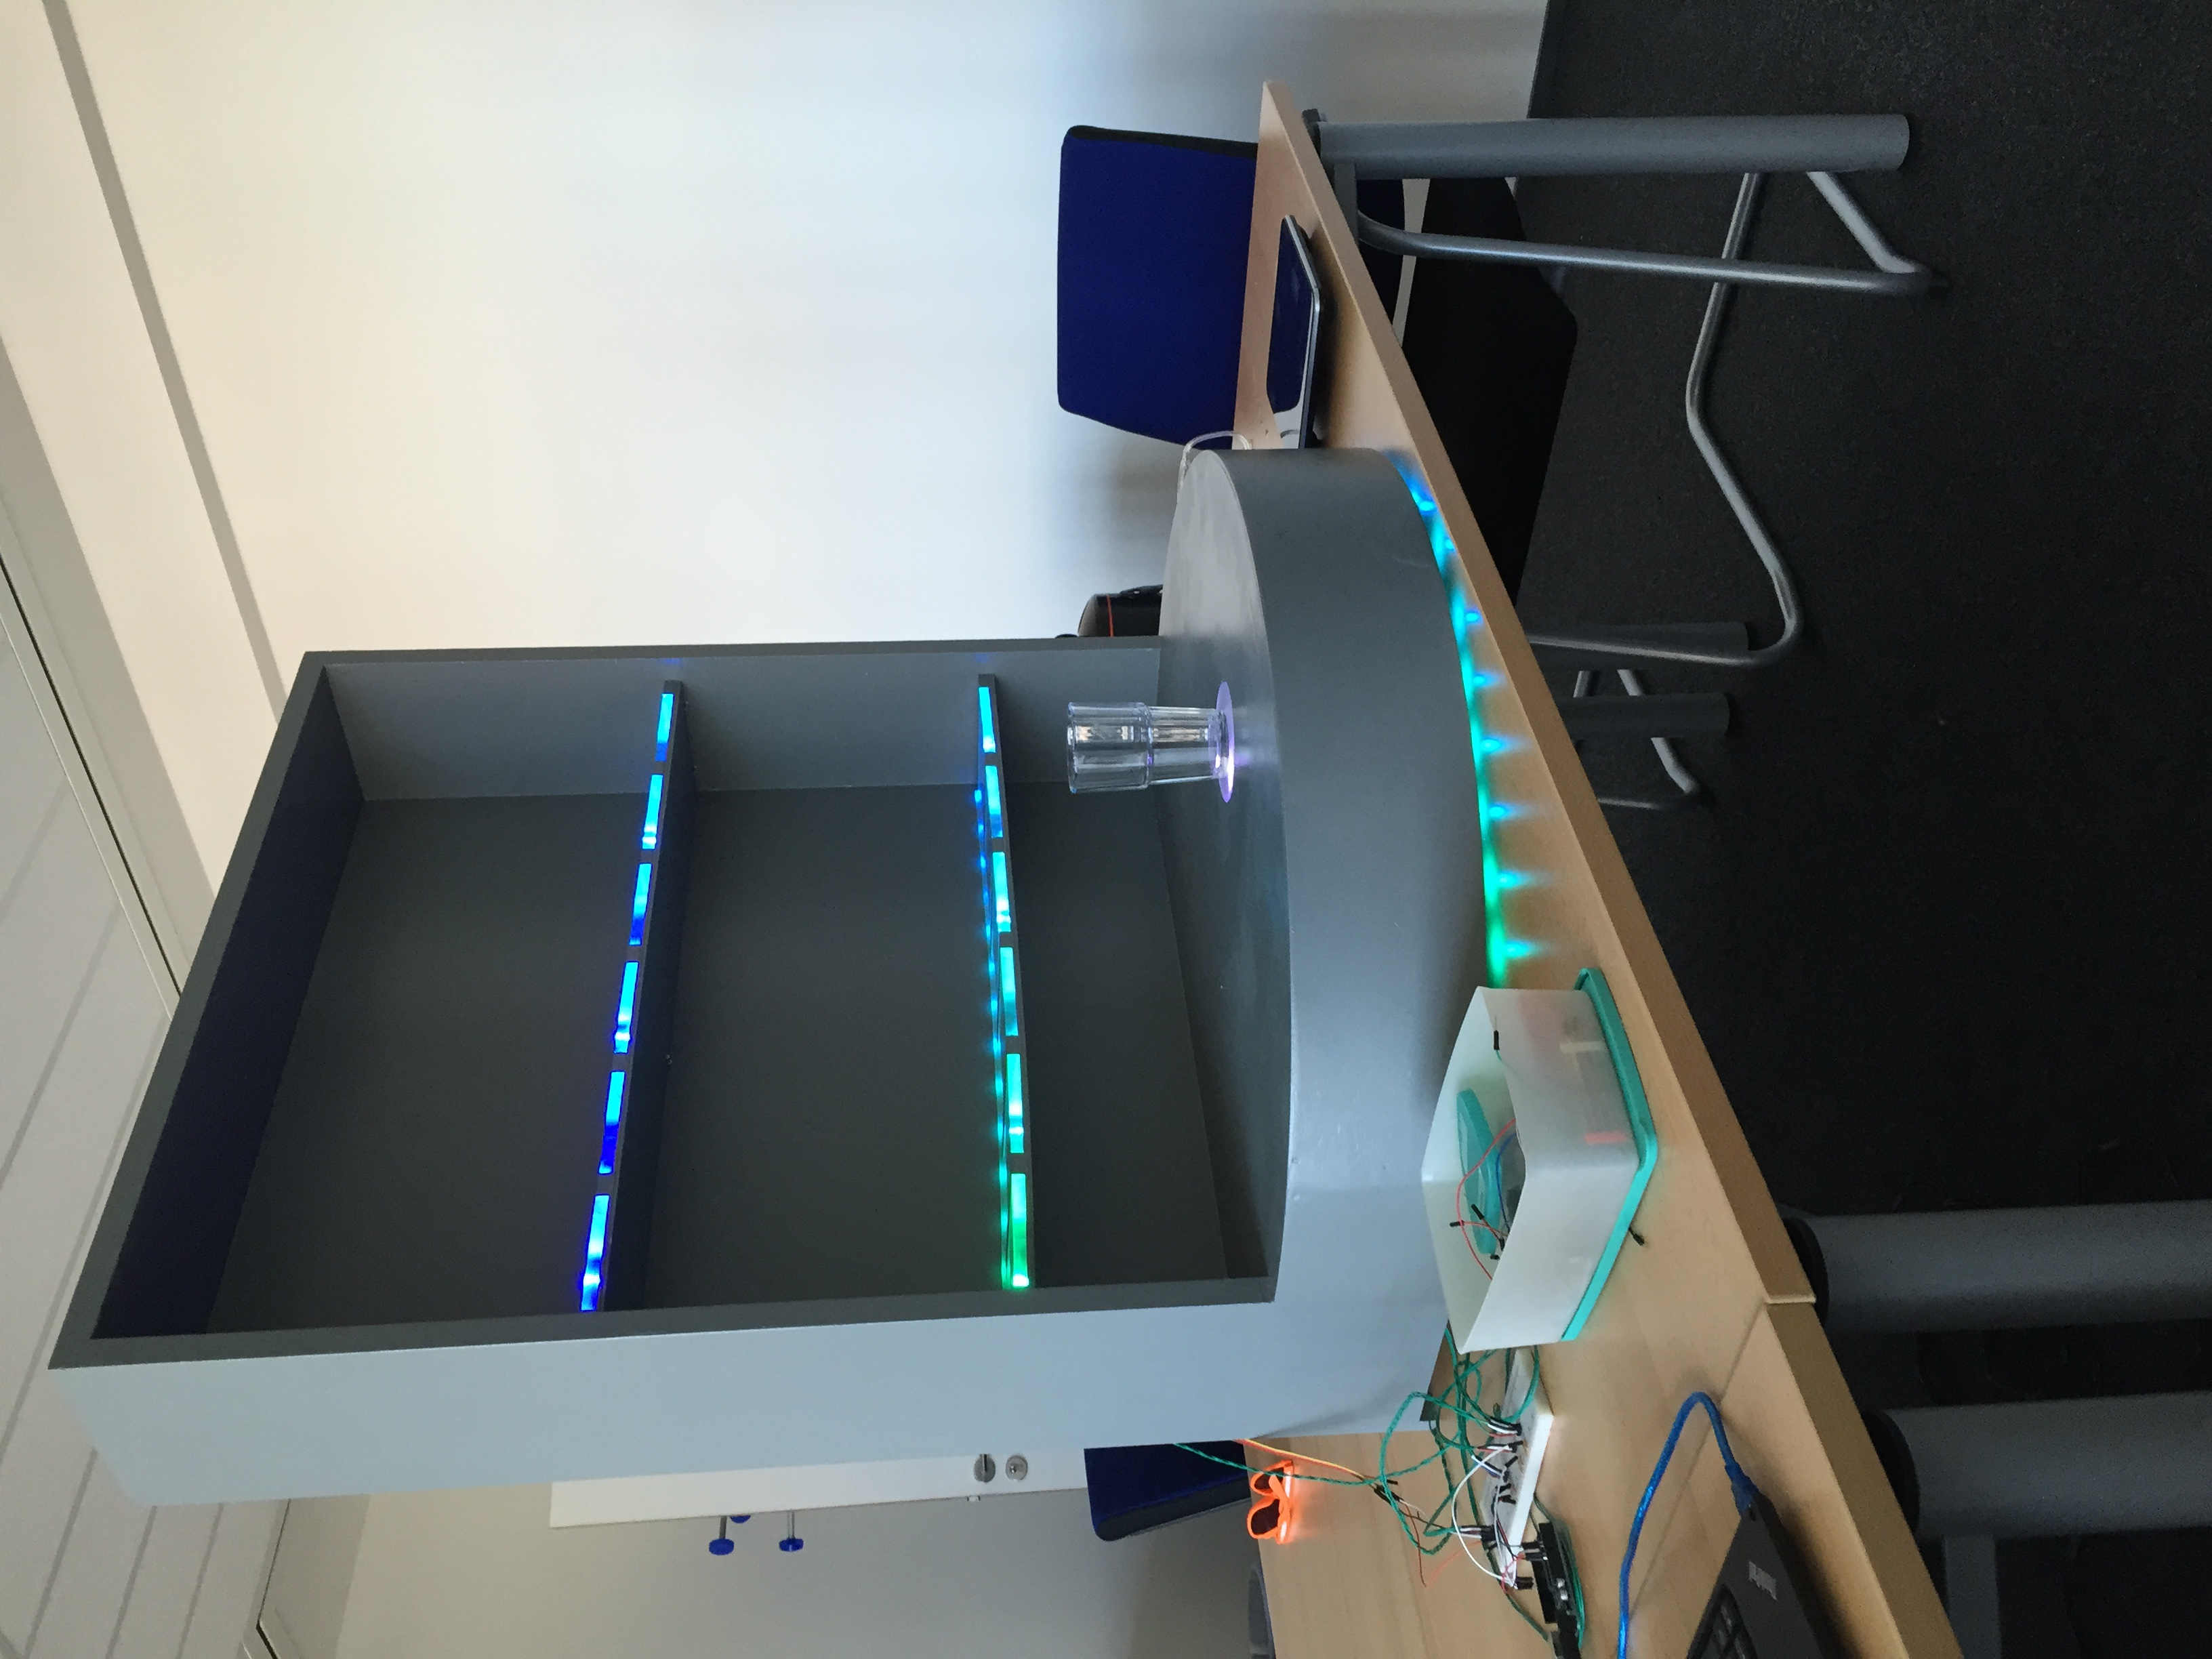
\includegraphics[width=0.5\linewidth]{pictures/illuminated_shelves.jpg}}
\captionof{figure}{Illumination of the shelves}\label{fig:illuminated_shelves}%      only if needed  
\end{minipage}


In the new design the plexiglass plates we cut into smaller pieces and put little pieces of wood between them. Furthermore we put a plate of wood under each shelve. This prevented the scattering of the light.\\
Figure \ref{fig:illuminated_shelves} shows who one bottle in bar can be lighted with the new design.

\subsection{Soldering and Wiring}
Finally we needed to connect all electronic parts together. The Raspberry Pi and the Arduino Uno are connected via an standard USB cable. Both have an individual 5 Volt power adapter with 1.2 Ampere for both devices. We have 5 LED stripes: One for both shelves, one for the glasses, one for the shaker and the ice, one for the glass panel above the scale and one for floor illumination. Each stripe needs three connections, one to ground, one to 5 Volt and one data connection to a digital pin the Arduino board. The scale is connected to a weighting module which is also connected to ground and 5 Volt and additional to 2 analog inputs on the Arduino board.

\begin{figure}[htbp] 
  \centering
     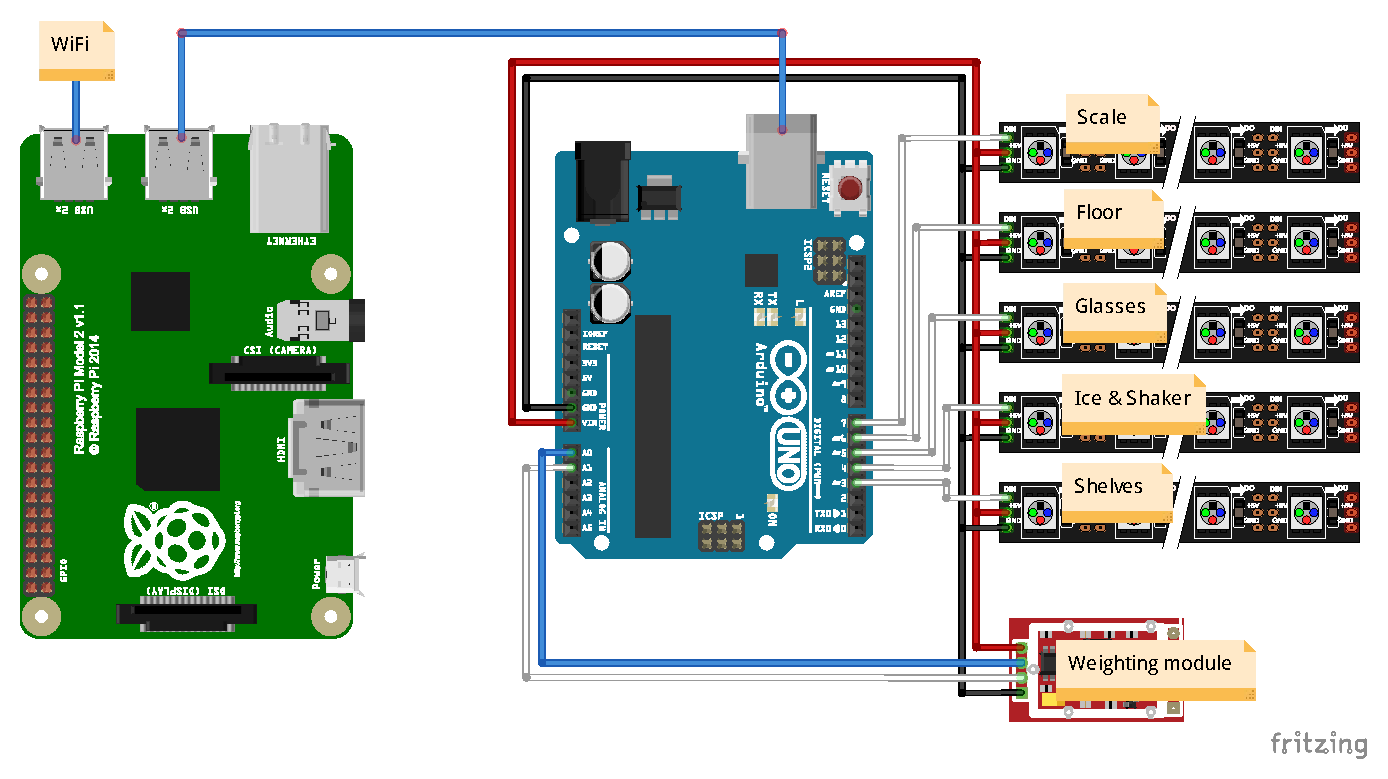
\includegraphics[width=1\linewidth]{pictures/sketch.pdf}
  \caption{Wiring sketch of the bar. The power adapters are not depicted. Made with Fritzing.}
  \label{fig:fritzing}
\end{figure}

All cables are equipped with plugs for easier assembling. For the LED stripes they were neccesary as the stripes doesn't fit through the drill holes. The cables from the stripes and the weighting module are all plugged into a self-soldered circuit board, which itself connects to the Arduino with only 3 plugs. 

\begin{figure}[htbp] 
  \centering
     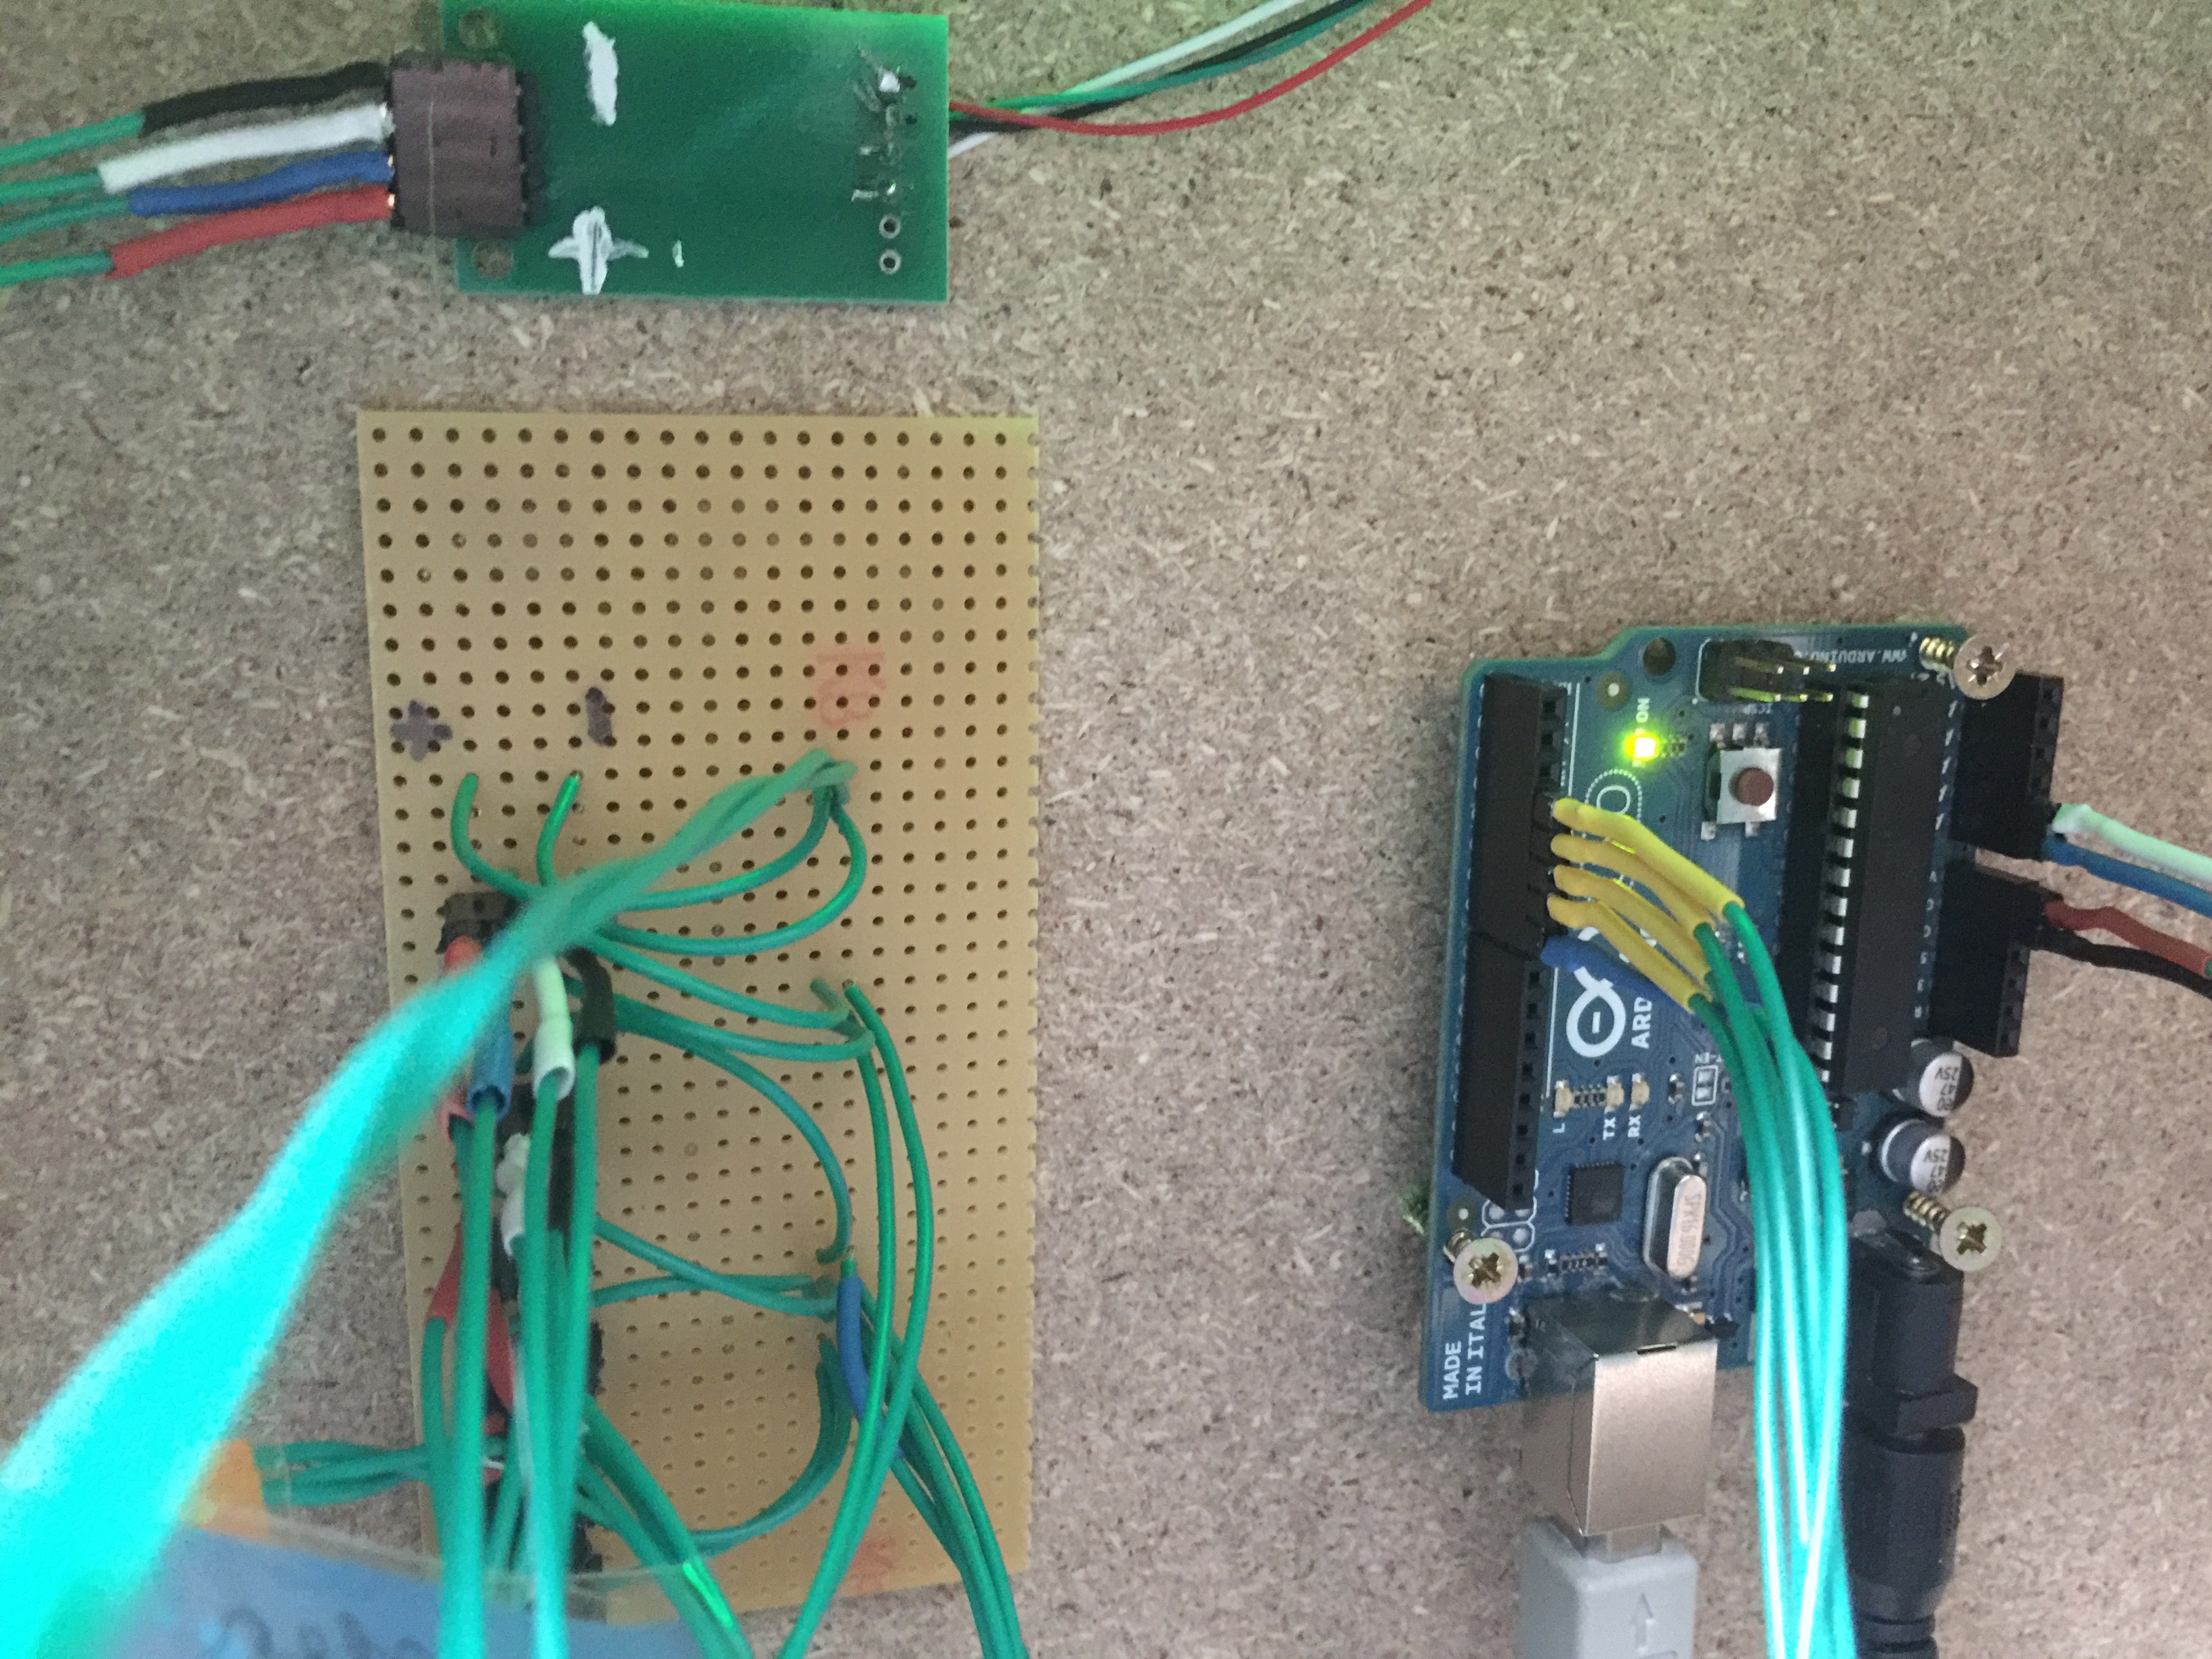
\includegraphics[width=1\linewidth]{pictures/built_in_electronic.JPG}
  \caption{View from below: On the top left is the weighting module. On the bottom left is the circuit board where all LED stripes and the weighting module are connected to and which connects to the Arduino on the right.}
  \label{fig:viewfrombelow}
\end{figure}


\section{Software Construction}
\subsection{Raspberry Pi and Arduino}
\subsection{Webserver}\label{sec:webserver}

\subsection{Database}
We used internal Django interface to build the database. For development, we used SQLite3 and later on we switched to MySQL because SQLite3 cannot handle multiple accesses to the database. Because we use Django it is very easy to switch. All tables are saved as models and we only need to create the internal database. Django is also able to import the data from SQLite3 into MySQL. \\
To create tables in Django, models are used. A model declares the column names, the corresponding types and constrains. Then Django need to migrate the database with the following commands:
\begin{lstlisting}[language=bash]
 $ python manage.py makemigrations
 $ python manage.py migrate
\end{lstlisting}
While the server is running we can access '127.0.0.1/admin/' to enter entries into the created tables. We also could to this with normal SQL commands. Now we can select the table and add new entries (Figure \ref{fig:db_entry}). \\
\begin{figure}[htbp] 
 \centering
    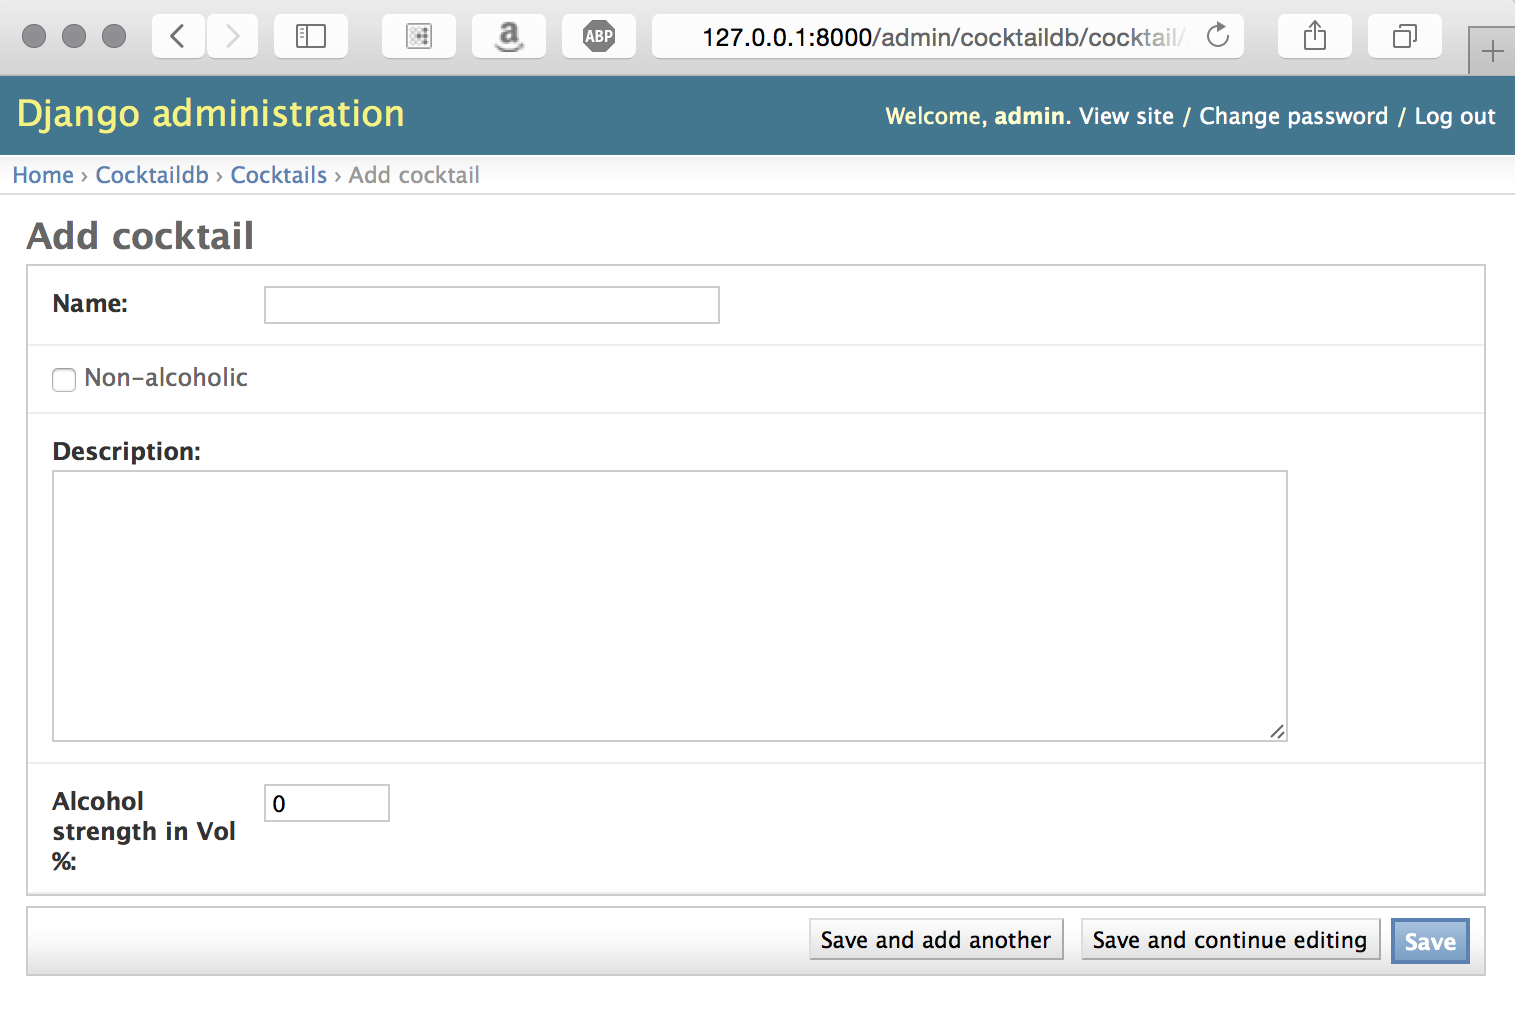
\includegraphics[width=0.7\linewidth]{pictures/db_insert_entry.png}
 \caption{Insert a new cocktail}
 \label{fig:db_entry}
\end{figure}
Django can handle all kinds of requests so that we do not need the normal SQL statements to ask for entries.

\subsection{Communication}
To communicate between the Arduino and the Raspberry Pi we use a python script, which is started when the Raspberry Pi boots. It connects to the database and to the Arduino. We used a sym link to have a fixed name to connect to the Arduino. It also opens the browser. \\
The script runs as long as the Raspberry Pi is not shut down. It waits for input from the database in form of a new cocktail order which is not done yet. In case we are in step 0, it sends a beginning message to the Arduino which waits for the first touch of the weight measuring module. Otherwise it select the first step of the current cocktail from the database and translate the step into a command which the Arduino can understand. The command consists always of nine characters and the first three encrypt the action. The next three characters can be empty or encrypt the ingredient. The last three characters can also be empty or encrypt the amount of an ingredient. If we need some information about time for mixing, shaking or filling the content of the shaker into a glass, we send it in the last six characters. \\
The Arduino always send an answer which can either be the message it received, 'READY' if an action has finished, 'TOUCHED' if someone touched the weight measuring module to start the process, 'NO\_INPUT' if no one touched the weight measuring module to start the process or 'ERROR' if the message lost some content. In case of an 'ERROR' message the message is sent again. In case of an 'NO\_INPUT' message the current order is deleted in the database.
\section{User Guide}
\subsection{Start the System}
To start the system you just need to connect the bar to the power supply system. After that the Raspberry Pi boots and when the 'Bar Dude' website is displayed, you can start ordering your cocktails. \\
To initialize the system you have to enter the current amount of each ingredient. After connecting to 'CocktailPi' discribed in the next subsection go to '192.168.0.1/admin/' and log in with 'admin' and 'ubercocktail'. Then select 'Ingredients' and edit the amount. You also should do this when you replace a bottle.
 \subsection{Select a Cocktail}
You have to connect to the Access Point 'CocktailPi' and log in with the password 'CocktailPi'. Then go to '192.168.0.1' in your browser. Now you can see the interface where you can choose your cocktail. For more information about the website read section \ref{sec:webserver}. You choose your cocktail by clicking on the corresponding 'Do it dude!' button. You get a number to know which cocktail is your's.

\begin{minipage}{\linewidth}% to keep image and caption on one page
\makebox[\linewidth]{%        to center the image
  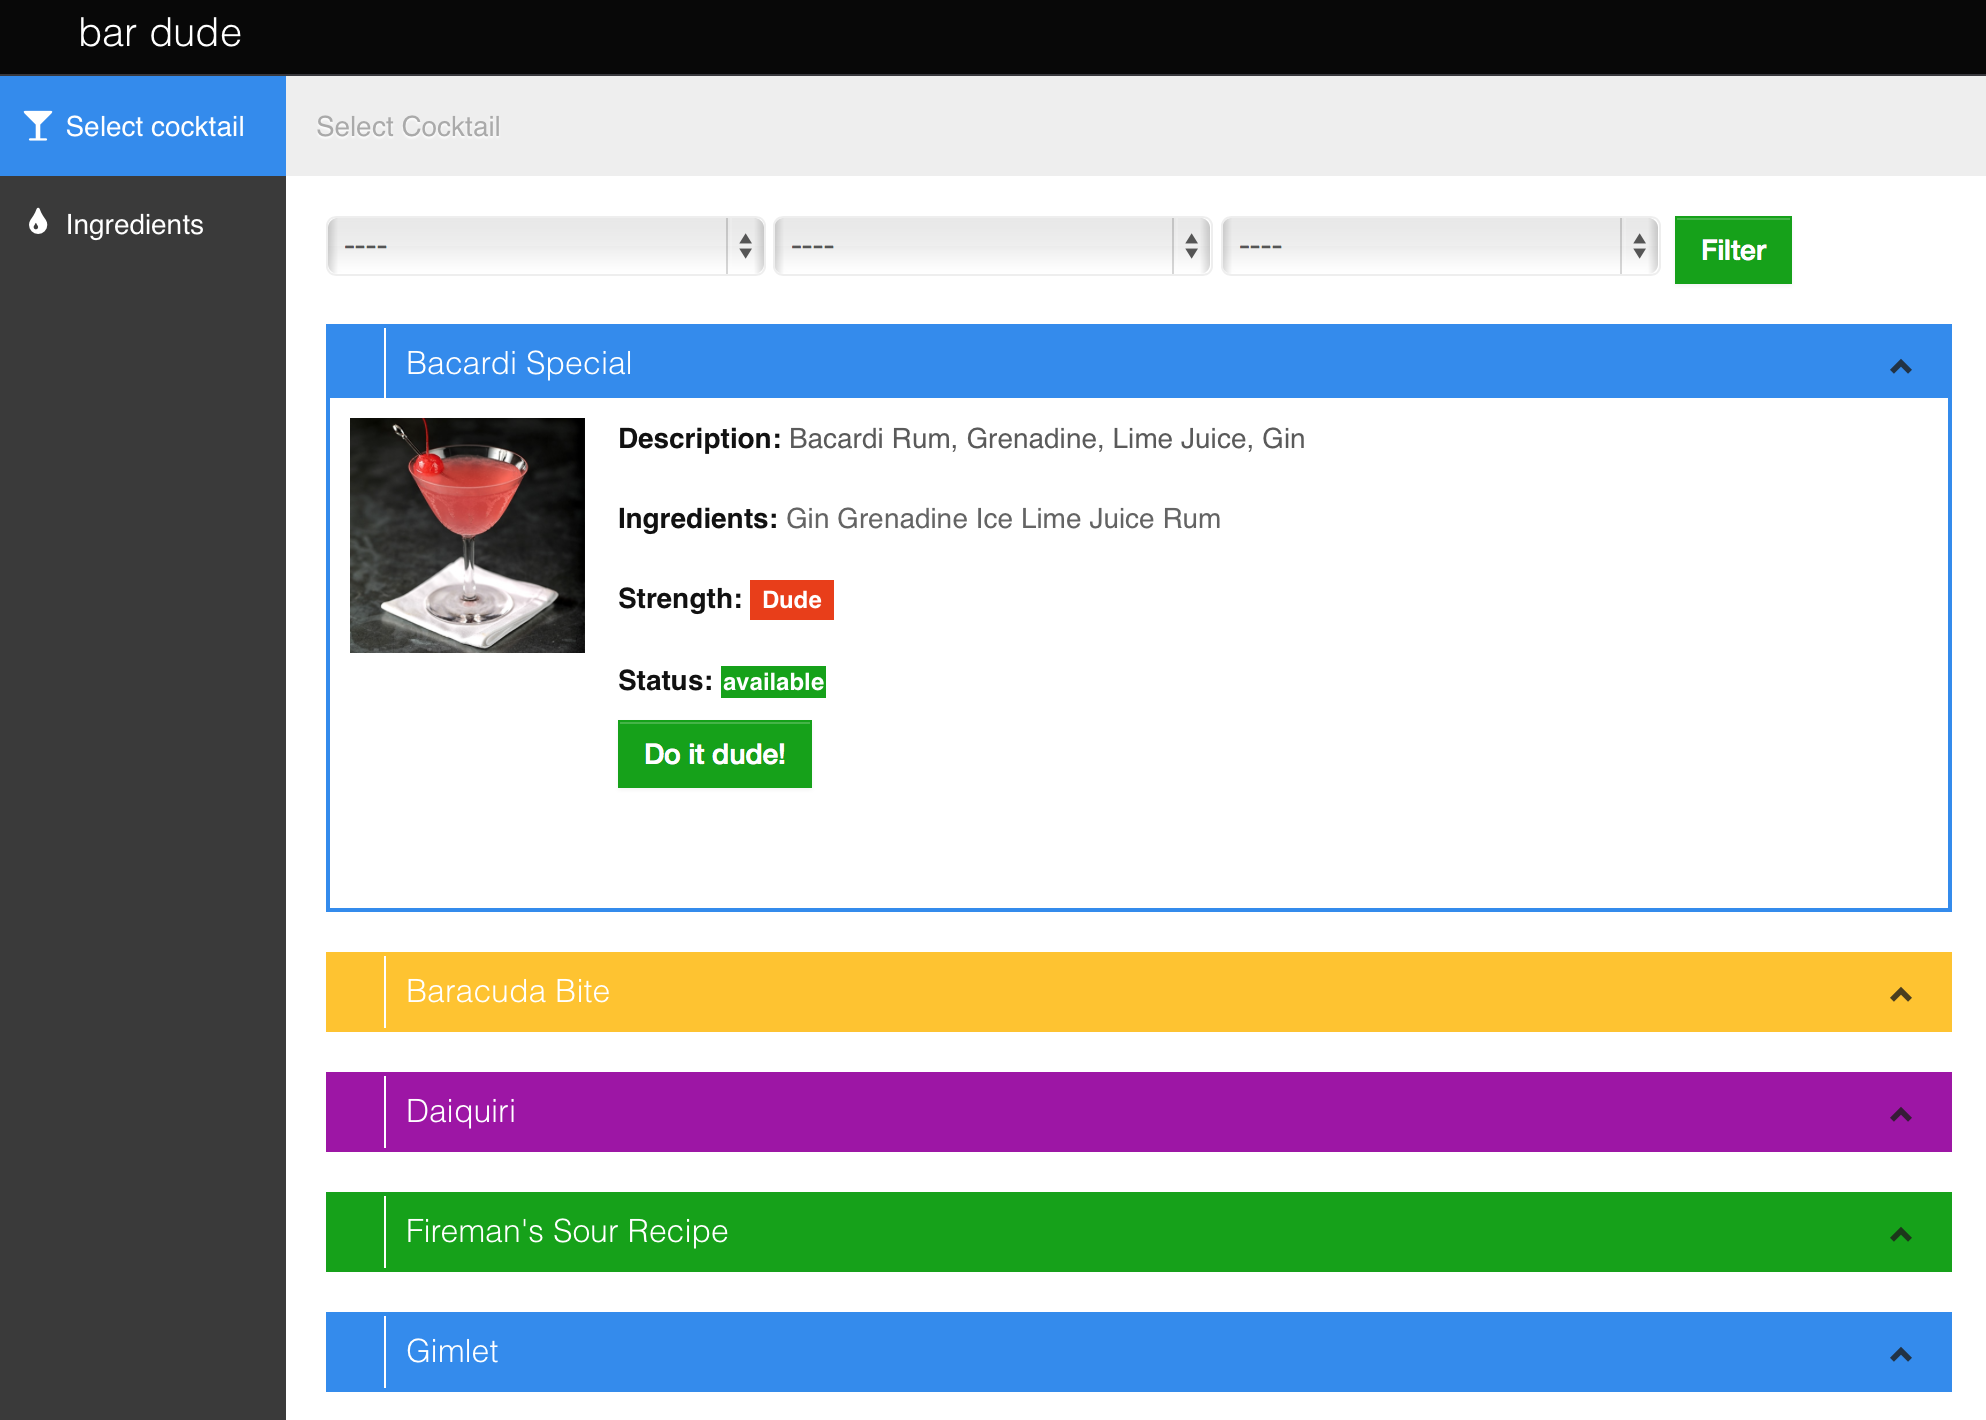
\includegraphics[width=0.8\linewidth]{pictures/select_cocktail.png}}
\captionof{figure}{Selection of a Cocktail}\label{fig:select_cocktail}%      only if needed  
\end{minipage}

 \subsection{Mix the Cocktail}
When your number is displayed on the display of the Raspberry Pi, you have 30 seconds to touch the weight measuring module. It also displays the countdown. If the time runs out, the order is deleted and the next cocktail number is displayed. \\
Now you can follow the instructions of the display. First you have to take a glass or a shaker depending on which is illuminated and put it on the weight measuring module. Then you add the illuminated ingredients. The weight measuring module shows you which amount if the ingredient is needed. It changes the color from red to green and the speed of the illumination slows down until you fill in enough. If you use a shaker you have to shake it when the bar goes wild. Then you have to take a glass and fill the content of the shaker into the glass. If you take a glass at first, you normally, not always, have to mix your cocktail. In this case the weight measuring module displays a circle. Take a spoon and mix until the next step is displayed. When your cocktail is finished, a party mode is displayed. 


\section{Conclusions}
%This paragraph will end the body of this sample document.
%Remember that you might still have Acknowledgments or
%Appendices; brief samples of these
%follow.  There is still the Bibliography to deal with; and
%we will make a disclaimer about that here: with the exception
%of the reference to the \LaTeX\ book, the citations in
%this paper are to articles which have nothing to
%do with the present subject and are used as
%examples only.
%\end{document}  % This is where a 'short' article might terminate

%ACKNOWLEDGMENTS are optional
%\section{Acknowledgments}
%This section is optional; it is a location for you
%to acknowledge grants, funding, editing assistance and
%what have you.  In the present case, for example, the
%authors would like to thank Gerald Murray of ACM for
%his help in codifying this \textit{Author's Guide}
%and the \textbf{.cls} and \textbf{.tex} files that it describes.
%
%%
%% The following two commands are all you need in the
%% initial runs of your .tex file to
%% produce the bibliography for the citations in your paper.
%\bibliographystyle{abbrv}
%\bibliography{sigproc}  % sigproc.bib is the name of the Bibliography in this case
%% You must have a proper ".bib" file
%%  and remember to run:
%% latex bibtex latex latex
%% to resolve all references
%%
%% ACM needs 'a single self-contained file'!
%%
%%APPENDICES are optional
%%\balancecolumns
%\appendix
%%Appendix A
%\section{Headings in Appendices}
%The rules about hierarchical headings discussed above for
%the body of the article are different in the appendices.
%In the \textbf{appendix} environment, the command
%\textbf{section} is used to
%indicate the start of each Appendix, with alphabetic order
%designation (i.e. the first is A, the second B, etc.) and
%a title (if you include one).  So, if you need
%hierarchical structure
%\textit{within} an Appendix, start with \textbf{subsection} as the
%highest level. Here is an outline of the body of this
%document in Appendix-appropriate form:
%\subsection{Introduction}
%\subsection{The Body of the Paper}
%\subsubsection{Type Changes and  Special Characters}
%\subsubsection{Math Equations}
%\paragraph{Inline (In-text) Equations}
%\paragraph{Display Equations}
%\subsubsection{Citations}
%\subsubsection{Tables}
%\subsubsection{Figures}
%\subsubsection{Theorem-like Constructs}
%\subsubsection*{A Caveat for the \TeX\ Expert}
%\subsection{Conclusions}
%\subsection{Acknowledgments}
%\subsection{Additional Authors}
%This section is inserted by \LaTeX; you do not insert it.
%You just add the names and information in the
%\texttt{{\char'134}additionalauthors} command at the start
%of the document.
%\subsection{References}
%Generated by bibtex from your ~.bib file.  Run latex,
%then bibtex, then latex twice (to resolve references)
%to create the ~.bbl file.  Insert that ~.bbl file into
%the .tex source file and comment out
%the command \texttt{{\char'134}thebibliography}.
%% This next section command marks the start of
%% Appendix B, and does not continue the present hierarchy
%\section{More Help for the Hardy}
%The acm\_proc\_article-sp document class file itself is chock-full of succinct
%and helpful comments.  If you consider yourself a moderately
%experienced to expert user of \LaTeX, you may find reading
%it useful but please remember not to change it.
%\balancecolumns
% That's all folks!
\end{document}
